\documentclass[12pt]{article}
\usepackage{amsfonts}
\usepackage{amsmath}
\usepackage[utf8]{inputenc}
\usepackage[italian]{babel}
\usepackage{geometry}
\usepackage{graphicx}
\usepackage{helvet}
\usepackage{float}
\graphicspath{ {./png/} }
\geometry{margin=1in}
\newcommand*{\N}{\mathbb{N}}
\title{ \LARGE\textbf{New Online Algorithms for Story Scheduling in Web Advertising}}
\date{}
\begin{document}
\maketitle
\section{Introduzione}
L’ambito di studio è lo storyboarding in cui gli inserzionisti desiderano presentare sequenze di ads (storie) senza interruzioni su una posizione di rilievo di una pagina web. Queste storie/jobs arrivano “online” e vengono attivate in base alla cronologia di navigazione dell'utente che, in ogni momento, continua a navigare con probabilità $\beta$. Nello storyboarding un singolo inserzionista controlla una posizione pubblicitaria di rilievo per un certo continuativo periodo di tempo. L’inserzionista crea una storia pubblicizzando i propri prodotti e la mostra utilizzando gli slot di tempo a lui concessi. Tipicamente molti inserzionisti competono per tale posizione. L’obiettivo di un ad server è quello di costruire uno schedule che massimizzi il risultato aspettato. 

In questo documento verranno introdotti degli algoritmi per la risoluzione del problema dello storyboarding, proposti da Susanne Albers e Achim Passen in una pubblicazione [1]. Tali algoritmi sono online, ovvero algoritmi che devono fornire dei risultati pur non avendo a disposizione, inizialmente, alcuni dei dati in ingresso. Più precisamente, l'algoritmo riceve in ingresso una generica sequenza $\sigma$ di input di cui, per ogni termine $\sigma_{i}$, deve fornire una risposta o prendere una decisione, basandosi solo sugli input ricevuti fino a tale istante, $\sigma_{j}$ con $j \leq i$. A questa tipologia si contrappone la definizione di algoritmo offline che designa i classici algoritmi, i quali possiedono tutti i dati d'ingresso fin dall'inizio dell'elaborazione, ovvero tutta la sequenza $\sigma$ [2].

Formalmente lo storyboarding è stato formulato come un problema di scheduling di jobs online da Dasgupta, Ghosh, Nazerzadeh e Raghavan in una pubblicazione [3]. Consideriamo un utente che al tempo $t = 0$ inizia una sessione web. Il tempo è “slotted”, cioè diviso in intervalli di tempo della stessa durata. In qualsiasi momento l’utente continua a navigare con probabilità $\beta$ e smette di navigare con probabilità $1 - \beta$ con $0 < \beta \leq 1$. Quindi il tempo di navigazione è una variabile casuale geometrica (distribuzione geometrica). Nel tempo le storie (jobs) arrivano online. Ogni job $i$ è specificato da un tempo di arrivo $a_{i}$, una lunghezza $l_{i}$, che rappresenta la lunghezza della storia, e un valore per unità $v_{i}$, che rappresenta il premio ottenuto dal server mostrando un unità del job $i$. Considerando tutti i jobs in arrivo si ottiene un'istanza del problema $I = (a_{i}, v_{i}, l_{i})_{i=1}^{N}$ con  $N \in \N \cup \{ \infty \}$.

Uno schedule $S$ per $I$ specifica quali job processare ad ogni tempo $t \geq 0$. $S$ può anche non contenere tutti i job di $I$, è infatti permesso tralasciare dei job non desiderati. $S$ è ben definito se ogni job schedulato è processato a tempi $t \geq a_{i}$ per al massimo $l_{i}$ unità di tempo. Inoltre il pre-abbandono dei jobs è permesso, cioè un job $i$ può essere processato per meno di $l_{i}$ unità di tempo. In questo caso non si può ottenere valore per la porzione pre-abbandonata non schedulata di un job. 

Dato uno schedule $S$, il suo valore è definito come il valore atteso $\sum_{t=0}^{\infty} \beta^{t}\cdot v(t)$ dove $v(t)$ è il valore per unità del job schedulato al tempo $t$. Sia $ALG$ un algoritmo online che, dato qualsiasi input $I$, costruisca uno schedule di valore $ALG(I)$. Sia $OPT(I)$ il valore di uno schedule ottimale offline per $I$. Si dice che $ALG$ è c-competitivo se esiste una costante $\alpha$ tale che $c \cdot ALG(I) + \alpha \geq OPT(I)$, $\forall I$ [4].

\section{Lavori precedenti}
Secondo quanto pubblicato da Susanne Albers e Achim Passen [1], lo storyboarding è stato studiato, da un punto di vista algoritmico, solamente da Dasgupta et al. [3]. Una prima osservazione è che se $\beta  = 1$ allora il problema è semplice da risolvere in quanto il valore dello schedule non dipende dal tempo in cui vengono eseguiti i vari job. Quindi ci si concentra sul caso in cui $0 < \beta < 1$.
Dasgupta et al. [1] hanno mostrato che nessun algoritmo deterministico online può avere un rapporto competitivo di $\beta + \beta^{2}$ che quindi è limitato superiormente da 2. Come risultato principale Dasgupta et al. hanno sviluppato un algoritmo greedy che è 7-competitivo. Inoltre hanno affrontato un’estensione del problema in cui i jobs hanno un valore per unità crescente anziché costante e in cui il valore è ottenuto solo quando il job è completamente finito. Infine hanno studiato un’altra estensione del problema in cui un job dev’essere schedulato immediatamente all’arrivo, altrimenti è perso.

\section{Contributi di questo documento}
Come detto in precedenza, Albers e Passen, in una pubblicazione [1], hanno presentato tre nuovi algoritmi online per lo storyboarding. Tutte le strategie seguono il paradigma del processare una data sequenza di job $I$ in fasi, in cui una fase consiste in k intervalli di tempi consecutivi per qualche $k\in \N$. 
Sia $k \geq 1$ un intero, una k-fase consiste in k intervalli di tempo consecutivi. Nello specifico l’n-esima k-fase $P_{n}$ è la sottosequenza di intervalli di tempo $(n-1)k,…,nk - 1$, per ogni $n \geq 1$. All’inizio di ogni fase un algoritmo crea uno schedule per la fase, ignorando i job che potrebbero arrivare durante la fase. In questo modo le decisioni di scheduling vengono prese una volta ogni tanto ed è come se, durante ogni singola fase, l'algoritmo lavorasse offline.

Il primo algoritmo presentato crea uno schedule ottimale per ogni fase e pre-abbandona i jobs che non hanno finito la loro esecuzione alla fine della rispettiva fase. Viene dimostrato che il rapporto competitivo di questa strategia è esattamente $1/\beta^{k-1}\cdot(1-\beta^{k}), \forall \beta$ e $\forall k \in \N$. Inoltre con la migliore scelta di k si ottiene una competitività di $4/(2 - \beta)$ che è limitata superiormente da 4, $\forall \beta$ e $\forall k \in \N$. Infine se scegliamo $k = 1$, l’algoritmo risultante è $1/(1-\beta)$ competitivo e tale scelta permette di ottenere migliori limitazioni della competitività per $\beta$ piccoli, cioè per $\beta < 2/3$.

Il secondo algoritmo presentato è un raffinamento del primo algoritmo che preferisce non pre-abbandonare i jobs che non sono terminati alla fine della rispettiva fase ma invece prova a rieseguirli nella fase successiva. Il rapporto competitivo di questa strategia è limitato superiormente da $1/\beta^{k-1} \cdot max\{1/\beta^{k-1}, 1/(1 - \beta^{2k} ), 1 + \beta^{3k}/(1 - \beta^{k} )\}$. Inoltre con la migliore scelta di k, otteniamo un fattore competitivo di $c = 1 + \phi$, dove $\phi = (1 + \sqrt{5})/2$ è la sezione aurea. Si ottiene quindi $c \approx 2.618$ che è molto vicino al limite teorico di 2 presentato da Dasgupta et al. [1] per un $\beta$ generico.

Il terzo algoritmo presentato è una generalizzazione del primo in cui si presuppone che ci siano m macchine parallele (ad positions) disponibili. In questo caso il valore dello schedule creato è dato da $\sum_ {t = 0}^{\infty}\sum_{j = 1}^{m}\beta^{t}\cdot v(t,j)$, dove $v(t,j)$ è il valore unitario del job schedulato sulla macchina $j$ al tempo $t$. Viene dimostrato che, per la migliore scelta di k, il rapporto competitivo di questa strategia è $(1 + 1/(1 - \beta(2 - \sqrt{2}))/(2 - \sqrt{2})$. Il rapporto è limitato inferiormente da $2/(2-\sqrt{2}) \approx 3.414$ e limitato superiormente da $1/(3 - 2\sqrt{2}) \approx 5.828$.

In questo documento, per ciascun algoritmo proposto da Albers e Passen, verrà descritta e discussa una relativa implementazione in codice Java. Inoltre verranno introdotte due implementazioni di due algoritmi offline necessari per effettuare un confronto con i relativi algoritmi online. Tutte le implementazioni sono state progettate al fine di poter ottenere il valore atteso di ciascun algoritmo. Infine verranno mostrati e commentati i risultati di alcuni test effettuati su ciascun algoritmo proposto, al fine di verificane empiricamente la competitività. I risultati saranno mostrati graficamente.

\section{$ALG1_{k}$}
Il primo algoritmo, chiamato $ALG1_{k}$, crea uno schedule ottimale per ogni k-fase $P_{n}$. Formalmente $ALG1_{k}$ funziona come segue. Diciamo che un job $i$ è disponibile al tempo $t$ se il job è arrivato entro $t$, cioè $a_{i} \leq t$ e non è stato mai schedulato ad un tempo qualsiasi $t’ < t$. Sia $Q_{n}$ l’insieme dei jobs disponibili all’inizio di $P_{n}$, cioè tutti quei job $i$ tali che $a_{i} \leq (n-1)k$. $ALG1_{k}$ ordina i job di $Q_{n}$ in ordine non crescente di valore unitario. I job che hanno lo stesso valore unitario vengono ordinati in ordine crescente di tempo di arrivo. A questo punto $ALG1_{k}$ assegna ad uno ad uno i job ordinati a $P_{n}$, finché tutti i $k$ intervalli di tempo vengono schedulati oppure la sequenza di jobs finisce. Se l’ultimo job schedulato non termina al termine di $P_{n}$, viene pre-abbandonato. $ALG1_{k}$ esegue questo schedule per $P_{n}$, ignorando i jobs che potrebbero arrivare durante la fase a tempi $t = (n-1)k + 1,…, nk - 1$. 

Adesso verranno introdotti alcuni teoremi e corollari ideati e dimostrati da Albers e Passen in una pubblicazione [1]. Le dimostrazioni dei seguenti enunciati sono consultabili nell'appendice A.
\newline\newline
\textbf{Teorema 1} (Competitività di $ALG1_{k}$): \textit{ $\forall k \in \N$ e $\forall \beta$, $ALG1_{k}$ è $1/(\beta^{k-1}(1 - \beta^{k}))$-competitivo.}
\newline \newline
\textbf{Corollario 1} (Determinazione del miglior valore di k)
\textit{Per $k = \lceil-log_{\beta} 2\rceil$, l'algoritmo risultante $ALG1_{k}$ è $4 / (2 - \beta )$-competitivo.} \newline\newline
Il teorema che segue dimostra che il rapporto competitivo di $ALG1_{k}$ mostrato sopra non può essere più piccolo.\newline\newline
\textbf{Teorema 2}
\textit{$\forall k \in \N$ e $\forall \beta$, il rapporto competitivo di $ALG1_{k}$ non è inferiore a $1 / (\beta^{k - 1} (1 - \beta^{k}))$.}\newline\newline
Combiniamo infine i Corollari 1 e 2 (Appendice A) per ottenere il seguente risultato.\newline\newline
\textbf{Corollario 3}
\textit{Impostando $k = 1$ se $\beta  \leq 2/3$ e $k = \lceil- log_{\beta}2\rceil$ altrimenti, otteniamo un algoritmo $ALG1_{k}$ che ottiene un rapporto competitivo di $min\{1 / (1 - \beta ), 4 / (2 - \beta )\}$.}

\section{$ALG2_{k}$}
Il secondo algoritmo, chiamato $ALG2_{k}$, è un raffinamento di $ALG1_{k}$; il principio di funzionamento è praticamente lo stesso. L’unica differenza sta nel fatto che tenta di ripristinare l’esecuzione di un eventuale job in una fase $P_{n}$ se è stato pre-abbandonato nella fase immediatamente precedente $P_{n-1}$. Formalmente $ALG2_{k}$ funziona in due step. \newline
Step(1): se $n > 1$, sia $i$ il job che è stato pre-abbandonato nella fase $P_{n-1}$. A questo punto definiamo il job residuo $r = (a_{i}, v_{i}, l_{r})$; $l_{r}$ è la parte rimanente del job $i$ che dev’essere processata. Aggiungiamo $r$ a $Q_{n}$. $ALG2_{k}$ ordina e schedula i job di $Q_{n}$ nello stesso modo di $ALG1_{k}$. Sia $S’(P_{n})$ lo schedule ottenuto in questo modo. \newline
Step(2): se $S’(P_{n})$ non contiene $r$ allora $S’(P_{n})$ è lo schedule finale per la fase. Altrimenti, se $S’(P_{n})$ contiene $r$ e tale job è schedulato per $s$ unità di tempo a partire dal tempo $t$, allora $ALG2_{k}$ modifica $S’(P_{n})$ in modo da schedulare $i$ per $s$ unità di tempo all’inizio della fase. Nello specifico il tempo di inizio di ogni job appartenente a $S’(P_{n})$ e diverso da $i$, viene aumentato di $s$ unità di tempo, mentre il tempo di inizio di $i$ diventa $t = (n-1)k$. Questo è lo schedule finale di $ALG2_{k}$ per $P_{n}$. 
Similmente a quanto fatto in Sezione 4, introduciamo un teorema e un corollario importanti. Le dimostrazioni dei seguenti enunciati sono consultabili nell'appendice A.
\newline\newline
\textbf{Teorema 3} (Competitività di $ALG2_{k}$)
\textit{$\forall k \in \N$ e $\forall \beta$, l'algoritmo $ALG2_{k}$ raggiunge un rapporto competitivo di $1 / \beta^{k - 1} \cdot max \{1 / \beta^{k - 1}, 1 / (1 - \beta^{2k}), 1 + \beta^{3k} / (1 - \beta^{k})\}$.}
\newline\newline
\textbf{Corollario 4} (Determinazione del miglior valore di k)
\textit{Sia $c = 1 + \phi$, dove $\phi = (1 + \sqrt{5}) / 2$ è la sezione aurea. Per $k = \lfloor -\frac{1}{2} log_{\beta} c \rfloor + 1$, $ALG2_{k}$ ottiene un rapporto competitivo di $c \approx 2.618.$}

\section{$ALG(m)_{k}$}
Il terzo algoritmo, chiamato $ALG(m)_{k}$, crea uno schedule ottimale per ogni k-fase $P_{n}$ considerando m macchine parallele. Formalmente $ALG(m)_{k}$ funziona come segue. Di nuovo, sia $Q_{n}$ l’insieme dei jobs $i$ che sono arrivati entro l’inizio di $P_{n}$, cioè $a_{i} \leq (n - 1)k$, e che non sono stati schedulati nelle fasi precedenti $P_{1}, … , P_{n}$. Per ogni $t = (n-1)k, … , nk - 1$ $ALG(m)_{k}$ determina gli m jobs che hanno il più alto valore unitario tra i jobs di $Q_{n}$ che non sono terminati al tempo t. Ognuno di questi è schedulato per una sola unità di tempo. Se un job era già stato schedulato al tempo $t-1$, allora viene assegnato alla stessa macchina al tempo $t$. Se, tra i jobs che non sono terminati di $Q_{n}$, l’m-esimo valore unitario più grande è $v$ ed esistono diversi jobs che hanno questo valore, allora viene data la precedenza a quei job che erano già stati schedulati precedentemente. I jobs non ancora iniziati invece vengono considerati in ordine crescente di tempo di arrivo. Se alla fine di $P_{n}$ ci sono jobs schedulati che non hanno terminato, vengono pre-abbandonati. $ALG(m)_{k}$ esegue questo schedule per $P_{n}$, ignorando i jobs che potrebbero arrivare durante la fase a tempi $t = (n-1)k + 1, …, nk - 1$.
Similmente a quanto fatto in Sezione 4, introduciamo un teorema e un corollario importanti. Le dimostrazioni dei seguenti enunciati sono consultabili nell'appendice A.
\newline \newline
\textbf{Teorema 4} (Competitività di $ALG(m)_{k}$)
\textit{$\forall k \in \N$ e tutte le probabilità $\beta$, $ALG(m)_{k}$ ottiene un rapporto competitivo di $\frac{1}{\beta^{k-1}}(1 + \frac{1}{1-\beta^{k}})$.}
\newline \newline
\textbf{Corollario 5} (Determinazione del miglior valore di k)
\textit{Per $k = \lceil log_{\beta} (2 - \sqrt{2})\rceil$, l'algoritmo risultante $ALG(m)_{k}$ ottiene un rapporto competitivo di $(1 + 1 / (1 - \beta (2 - \sqrt{2})) / (2 - \sqrt{2}).$}

\section{Implementazioni}
In questa sezione verranno mostrate e discusse delle possibili implementazioni  dei tre algoritmi precedentemente introdotti. Tali implementazioni sono state progettate al fine di poter ottenere il valore atteso di ciascun algoritmo, per poter verificare empiricamente i risultati ottenuti dalle analisi descritte sopra. Il linguaggio di programmazione utilizzato è Java. Inoltre sono state fatte le seguenti assunzioni: per ogni job $i$, $a_{i} \in \N$ mentre $v_{i}$ e $l_{i}$ sono interi positivi diversi da $0$. Le fasi sono numerate a partire da $0$. Per quanto riguarda $ALG(m)_{k}$, è stato assunto che $m$ sia un intero positivo maggiore o uguale a $1$. Inoltre ogni job è stato implementato attraverso la classe Job, contenente i seguenti campi:
\begin{itemize}
\item{int index, che rappresenta l’indice del job $i$;}
\item{int arrivalTime, che rappresenta il suo tempo di arrivo $a_{i}$;}
\item{int value, che rappresenta il suo valore unitario $v_{i}$;}
\item{int length, che rappresenta la sua lunghezza $l_{i}$.}
\end{itemize}

\subsection{Implementazione di $ALG1_{k}$}
L’algoritmo $ALG1_{k}$ è stato implementato attraverso la classe ALG1k. I suoi campi sono:
\begin{itemize}
\item{double beta, che rappresenta la probabilità $\beta$;}
\item{int k, che rappresenta la lunghezza di ciascuna fase;}
\item{LinkedList$<$Job$>$ totalJobs, che rappresenta l’insieme totale dei job $I$}
\item{LinkedList$<$Job$>$ activeJobs, che rappresenta l’insieme dei job disponibili in una certa fase $Q_{n}$}
\end{itemize}
Il suo unico costruttore ha come parametri k, beta e totalJobs. Il metodo “start” fa partire l’esecuzione dell’algoritmo e restituisce il valore atteso su input totalJobs, k e beta. In pratica, finché ci sono job da processare e per ogni fase $n$:
\begin{itemize}
\item{Rimuove dalla lista totalJobs i job che sono arrivati prima della fase $n$ e li inserisce nella lista activeJobs (metodo “scheduleActiveJobs”).}
\item{Ordina la lista activeJobs in ordine non-decrescente di valore unitario. I job che hanno lo stesso valore unitario  vengono ordinati in ordine crescente di tempi di arrivo (metodo “sortActiveJobs”). L’algoritmo di ordinamento utilizzato è il merge-sort.}
\item{Se activeJobs contiene almeno un elemento, estrae e rimuove il suo Job in testa $j$  e, per ogni $t$ compreso tra $nk$ e $k(n + 1) - 1$, somma $\beta^{t} * v_{j}$ al valore atteso calcolato fino al quel momento, decrementa $l_{j}$ di $1$ e, se $l_{j} = 0$ e $t \neq k(n + 1) - 1$, imposta $j$ come il job in testa ad activeJobs (se esiste), dopo averlo estratto e rimosso (metodo “processPhase”).}
\end{itemize}

\subsection{Implementazione di $ALG2_{k}$}
L’algoritmo $ALG2_{k}$ è stato implementato attraverso la classe ALG2k. I suoi campi sono:
\begin{itemize}
\item{double beta, che rappresenta la probabilità $\beta$;}
\item{int k, che rappresenta la lunghezza di ciascuna fase;}
\item{LinkedList$<$Job$>$ totalJobs, che rappresenta l’insieme totale dei job $I$}
\item{LinkedList$<$Job$>$ activeJobs, che rappresenta l’insieme dei job disponibili in una certa fase $Q_{n}$}
\item{Job interruptedJob, che rappresenta l’eventuale job da dover ripristinare in una determinata fase.}
\end{itemize}
Il suo unico costruttore ha come parametri k, beta e totalJobs. Il metodo “start” fa partire l’esecuzione dell’algoritmo e restituisce il valore atteso su input totalJobs, k e beta. In pratica, finché ci sono job da processare e per ogni fase $n$:
\begin{itemize}
\item{Rimuove dalla lista totalJobs i job che sono arrivati prima della fase $n$ e li inserisce nella lista activeJobs (metodo “scheduleActiveJobs”).}
\item{Ordina la lista activeJobs in ordine non-decrescente di valore unitario. I job che hanno lo stesso valore unitario  vengono ordinati in ordine crescente di tempi di arrivo (metodo “sortActiveJobs”). L’algoritmo di ordinamento utilizzato è il merge-sort.}
\item{Se activeJobs contiene almeno un elemento, estrae e rimuove a uno a uno i job in testa ad activeJobs e li inserisce in una lista S finché non ci sono più job da estrarre oppure se la somma delle lunghezze dei job estratti è maggiore o uguale a k. A questo punto, se tra i job di S è presente interruptedJob, viene rimosso e reinserito in testa ad S. Se la somma delle lunghezze dei job in S è superiore a k e se interruptedJob è l’ultimo in S e non è l’unico in S, allora la sua lunghezza viene ridotta in modo tale che la somma delle lunghezze di tutti i job presenti in S sia uguale a k. Se invece interruptedJob non era presente in S ma era tra i job appartenenti ad activeJobs, allora viene rimosso da quest’ultima lista (metodo “createSchedule”).}
\item{Se S contiene almeno un elemento, finché S non è vuoto, estrae e rimuove il suo Job in testa $j$  e, per ogni $t$ a partire da $kn$, somma $\beta^{t} * v_{j}$ al valore atteso calcolato fino al quel momento e decrementa $l_{j}$ di $1$ finché $t \geq k(n + 1) - 1$ o $l_{j} = 0$. Se si verifica una delle due condizioni allora controlla se $t \geq k(n + 1) - 1$ e se  $l_{j} \neq 0$. In tal caso impostata interruptedJob $= j$ lo aggiunge ad activeJobs. (metodo “processPhase”).}
\end{itemize}

\subsection{Implementazione di $ALG(m)_{k}$}
L’algoritmo $ALG(m)_{k}$ è stato implementato attraverso la classe ALGmk. I suoi campi sono:
\begin{itemize}
\item{double beta, che rappresenta la probabilità $\beta$;}
\item{int m, che rappresenta il numero di macchine $m$;}
\item{int k, che rappresenta la lunghezza di ciascuna fase;}
\item{LinkedList$<$Job$>$ totalJobs, che rappresenta l’insieme totale dei job $I$}
\item{LinkedList$<$Job$>$ activeJobs, che rappresenta l’insieme dei job disponibili in una certa fase $Q_{n}$}
\end{itemize}
Il suo unico costruttore ha come parametri k, m, beta e totalJobs. Il metodo “start” fa partire l’esecuzione dell’algoritmo e restituisce il valore atteso su input totalJobs, k, m e beta. In pratica, finché ci sono job da processare e per ogni fase $n$:
\begin{itemize}
\item{Rimuove dalla lista totalJobs i job che sono arrivati prima della fase $n$ e li inserisce nella lista activeJobs (metodo “scheduleActiveJobs”).}
\item{Ordina la lista activeJobs in ordine non-decrescente di valore unitario. I job che hanno lo stesso valore unitario  vengono ordinati in ordine crescente di tempi di arrivo (metodo “sortActiveJobs”). L’algoritmo di ordinamento utilizzato è il merge-sort.}
\item{Crea un array di m elementi chiamato machines e in ciascuna posizione a partire dalla prima inserisce i primi job di activeJobs, dopo averli estratti e rimossi, finché possibile. A questo punto, per ogni $t$ compreso tra $nk$ e $k(n + 1) - 1$, accede ad ogni elemento di machines a partire dal primo fino all’ultimo disponibile e, per ciascun job $j$ (se presente), somma $\beta^{t} * v_{j}$ al valore atteso calcolato fino al quel momento e decrementa $l_{j}$ di $1$. Se a questo punto $l_{j} = 0$, se $t$ non è l’ultimo tempo della fase $n$ e activeJobs contiene almeno un elemento, allora estrae e rimuove l’elemento in testa di activeJob e lo sostituisce alla posizione di machines in cui si trovava $j$, altrimenti rimuove $j$ da tale posizione (metodo “processPhase”).}
\end{itemize}

\subsection{Implementazione di $CHOP$}
L’algoritmo $ALG2_{k}$ è stato implementato attraverso la classe ALG2k. I suoi campi sono:
\begin{itemize}
\item{double beta, che rappresenta la probabilità $\beta$;}
\item{int k, che rappresenta la lunghezza di ciascuna fase;}
\item{LinkedList$<$Job$>$ totalJobs, che rappresenta l’insieme totale dei job $I$}
\end{itemize}
Il suo unico costruttore ha come parametri k, beta e totalJobs. Il metodo “start” fa partire l’esecuzione dell’algoritmo e restituisce il valore atteso su input totalJobs, k e beta. All'inizio trasforma l'input iniziale totalJobs in un input k-quantizzato attraverso il metodo ''quantizeTotalJobs'' e li ordina in ordine non-decrescente di valore unitario. I job che hanno lo stesso valore unitario  vengono ordinati in ordine crescente di tempi di arrivo (metodo “sortActiveJobs”). L’algoritmo di ordinamento utilizzato è il merge-sort. A questo punto, finché totalJobs non è vuota e a partire da un intero $t = 0$, estrae e rimuove dalla lista totalJobs il primo job $j$ che trova disponibile (se esiste), ovvero tale che il suo tempo di arrivo sia minore o uguale a $t$ e somma $\beta^{t} * v_{j}$ al valore atteso ottenuto fino a quel momento. Successivamente decrementa di uno la lunghezza di $j$ e, se la lunghezza attuale è maggiore di 0, lo riaggiunge alla lista totalJobs nella posizione precedente e incrementa di uno $t$.

\subsection{Implementazione di $OPT^{*}$}
L’algoritmo $OPT^{*}$ è stato implementato attraverso la classe OptStar. I suoi campi sono:
\begin{itemize}
\item{double beta, che rappresenta la probabilità $\beta$;}
\item{int m, che rappresenta il numero di macchine $m$;}
\item{int k, che rappresenta la lunghezza di ciascuna fase;}
\item{LinkedList$<$Job$>$ totalJobs, che rappresenta l’insieme totale dei job $I$}
\item{LinkedList$<$Job$>$ activeJobs, che rappresenta l’insieme dei job disponibili in una certa fase $Q_{n}$}
\end{itemize}
Il suo unico costruttore ha come parametri k, m, beta e totalJobs e a differenza di Algmk imposta m = 2*m. Il metodo “start” fa partire l’esecuzione dell’algoritmo e restituisce il valore atteso su input totalJobs, k, m e beta. All'inizio trasforma l'input iniziale totalJobs in un input k-quantizzato attraverso il metodo ''quantizeTotalJobs''. Successivamente, finché ci sono job da processare e per ogni tempo $t \geq 0$:
\begin{itemize}
\item{Rimuove dalla lista totalJobs i job che sono disponibili al tempo $t$ e li inserisce nella lista activeJobs (metodo “scheduleActiveJobs”).}
\item{Ordina la lista activeJobs in ordine non-decrescente di valore unitario. I job che hanno lo stesso valore unitario  vengono ordinati in ordine crescente di tempi di arrivo (metodo “sortActiveJobs”). L’algoritmo di ordinamento utilizzato è il merge-sort.}
\item{Finché activeJobs non è vuoto, estrae e rimuove il primo job $j$ da tale lista e somma $\beta^{t} * v_{j}$ al valore atteso ottenuto fino a quel momento. Successivamente decrementa di uno la lunghezza di $j$ e, se la lunghezza attuale è maggiore di 0, lo riaggiunge alla lista totalJobs. Il ciclo termina anche se sono stati processati $m$ job. Infine viene incrementato $t$ di uno}
\end{itemize}

\section{Simulazioni}
In questa sezione verranno mostrati i risultati ottenuti da alcune simulazioni effettuate sugli algoritmi precedentemente descritti. Lo scopo di tali simulazioni è quello di verificare empiricamente la validità dei teoremi dimostrati precedentemente. Ciascun algoritmo online è stato messo a confronto con un determinato algoritmo offline in base a determinate caratteristiche che verranno mostrate successivamente. La necessità di utilizzare tali algoritmi offline per il confronto nasce dall’impossibilità di determinare con certezza l’implementazione di un algoritmo offline ottimale per la risoluzione del problema dello storyboarding scheduling. Sono stati effettuati due tipi di simulazioni. La prima simulazione consiste nell'eseguire ciascun algoritmo su un input particolare in modo da massimizzare la perdita del valore ottenuto. La seconda invece consiste nel generare casualmente 1000 input composti da 100 job ed eseguire ciascun algoritmo su ogni singolo input. Ogni tipo di simulazione è stata divisa in quattro test. Ogni test rappresenta un particolare intervallo dei valori che $\beta$ può assumere, ovvero $0 < \beta < 1$. Gli intervalli scelti sono i seguenti:
\begin{itemize}
\item{$0 < \beta < 0.3$,}
\item{$0.4 \leq \beta < 0.6$,}
\item{$0.6 \leq \beta < 0.8$,}
\item{$0.8 \leq \beta < 1$.}
\end{itemize}
Quindi, per ogni test, vengono generati 1000 valori di $\beta$ appartenenti al relativo intervallo e, per ogni $\beta$, viene calcolata la lunghezza ottimale delle fasi ($k$) e il rapporto competitivo $c$. A questo punto per ogni coppia $\beta$, $k$ si calcola il valore ottenuto dell'algoritmo online e di quello offline per gli/l'input precedentemente generati/o. Tutti i risultati ottenuti vengono scritti in un file strutturato, in modo tale da poter essere letti ed analizzati in un momento successivo. Per ogni input viene calcolato il rapporto tra il valore dell'algoritmo offline (moltiplicato per un determinato valore che verra mostrato in seguito) e il valore dell'algoritmo online. Il rapporto calcolato non deve superare il rapporto competitivo dell'algoritmo online relativo. Nel caso del secondo tipo di simulazione, una volta calcolato questo valore per tutti gli input, se ne ricava il massimo. 

I risultati verranno mostrati tramite grafici bidimensionali in cui si associa ad ogni valore di $\beta$ (asse X) il rapporto o il massimo dei rapporti tra il valore dell'algoritmo online e di quello offline (asse Y). I grafici sono consultabili nell'appendice B.

\subsection{Test effettuati su $ALG1_{k}$}
Prima di mostrare i risultati ottenuti, occorre definire l’algoritmo offline utilizzato per il confronto. Tale algoritmo è $CHOP$, che è stato descritto in Appendice A.1 come l’algoritmo che permette di riprendere l’esecuzione dei job interrotti in un momento successivo. Per qualsiasi input, in qualsiasi istante $t$, $CHOP$ schedula un job che ha il più alto valore per unità tra i job non completati che sono arrivati entro il tempo $t$. Vale dunque $CHOP(I_{k}) \geq OPT(I_{k})$. Inoltre dimostriamo il seguente corollario del Teorema 1.
\newline \newline
\textbf{Corollario del Teorema 1}
\textit{Per ogni input $I$ e ogni rispettivo input k-quantizzato $I_{k}$, $\forall k \in \N$ e per tutte le probabilità $\beta$ vale
$c \cdot ALG1_{k}(I) \geq OPT(I) \iff c \cdot ALG1_{k}(I) \geq 1/\beta^{k-1} CHOP(I_{k})$
 con $c = \frac{1}{\beta^{k-1}(1 - \beta^{k})}$.}
\newline \newline
\textit{Dimostrazione} 
Per il Lemma 1, $\forall k \in \N$ e per tutte le probabilità $\beta$, vale $$\frac{1}{\beta^{k-1}} OPT(I_{k}) \geq OPT(I).$$
Inoltre, durante la dimostrazione del Teorema 3, è stato dimostrato che $$\frac{1}{1 - \beta^{k}} ALG1_{k}(I) \geq CHOP(I_{k}).$$
Combinando queste due disequazioni otteniamo
$$OPT(I) \leq \frac{1}{\beta^{k-1}} OPT(I_{k}) \leq \frac{1}{\beta^{k-1}} CHOP(I_{k}) \leq \frac{1}{\beta^{k-1}(1 - \beta^{k})} ALG1_{k}(I) = c \cdot ALG1_{k}(I)$$
e dunque possiamo affermare che
\begin{equation}
c \cdot ALG1_{k}(I) \geq OPT(I) \iff c \cdot ALG1_{k}(I) \geq \frac{1}{\beta^{k-1}} CHOP(I_{k}) \tag*{$\square$}
\end{equation}

Grazie al risultato di questo corollario è possibile confrontare $ALG1_{k}$ su input $I$ con $CHOP$ su input $I_{k}$ per poter verificare che il rapporto competitivo di $ALG1_{k}$ sia effettivamente quello dimostrato, cioè $\frac{1}{\beta^{k-1}(1 - \beta^{k})}$. Per ogni $\beta$ è stata calcolata la lunghezza di fase $k$ con la funzione descritta nel Corollario 1. Per ciascun input il rapporto è stato calcolato come $\frac{1}{\beta^{k-1}} \cdot CHOP(I_{k}) / ALG1_{k}(I)$. Ciascun rapporto è stato confrontato con il relativo rapporto competitivo teorico. Adesso verranno mostrati e commentati i risultati ottenuti. Si ricorda che i grafici sono consultabili nell'appendice B.
\subsubsection{Test del rapporto massimo}
Commentiamo i risultati ottenuti. Osservando la Figura B.1.5, che mostra i risultati complessivi di tutti i test, possiamo affermare che i dati confermano il Teorema 1, in quanto nessuno dei rapporti massimi calcolati supera il relativo rapporto competitivo teorico.
Dal grafico della Figura B.1.1 notiamo che le due funzioni sono molto simili. Questo è dovuto al fatto che, in questo intervallo di $\beta$, la scelta della lunghezza di fase è $k=1$, per cui tutti i job disponibili per OPT ad un certo tempo t lo sono anche per $ALG1_{k}$. L'unico caso in cui il valore di $ALG1_{k}$ subisce una pertita si ha quando avviene il pre-abbandono di job.

Dalle successive figure (da B.1.2 a B.1.4) notiamo un aumento improvviso dei rapporti delle funzioni in corrispondenza ad alcuni valori di $\beta$. Questo è dovuto al cambio della lunghezza della fase $k$. Complessivamente notiamo che, al crescere di $\beta$, i rapporti massimi calcolati tendono a diminuire fino al successivo cambio di lunghezza di fase.

\subsubsection{Test del caso peggiore}
Descriviamo l'input $I$ utilizzato che rappresenta un caso pessimo. L'algoritmo offline utilizzato per il confronto viene eseguito su $I_{k}$, di conseguenza ciascun job disponibile al tempo $t$ per $CHOP$ lo è anche per $ALG1_{k}$. Per i primi $k$ istanti di tempo il valore ottenuto da $ALG1k_{k}$ è lo stesso di $CHOP$. Negli istanti di tempo successivi invece il valore di $ALG1_{k}$ può essere minore rispetto a quello ottenuto da $CHOP$ in quanto può avvenire il pre-abbandono di job. Di conseguenza, l'input peggiore consiste di un singolo job di lunghezza infinita con tempo di arrivo di $t = 0$. In questo modo, $ALG1_{k}$ pre-abbandona il job alla fine della prima fase e non ottiene più valore negli istanti successivi, al contrario di $CHOP$ che continua ad eseguire il job. Di seguito i risultati ottenuti.

In ciascun grafico (da Figura B.1.6 - a B.1.10) notiamo che ciascun rapporto calcolato è uguale al rispettivo rapporto competitivo teorico. Possiamo quindi affermare che i dati confermano il Teorema 1.
\subsection{Test effettuati su $ALG2_{k}$}
Anche per $ALG2_{k}$, l’algoritmo offline utilizzato per il confronto è $CHOP$. Vale infatti il seguente corollario del Teorema 3.
\newline\newline
\textbf{Corollario del Teorema 3}
\textit{Per ogni input $I$ e ogni rispettivo input k-quantizzato $I_{k}$, $\forall k \in \N$ e per tutte le probabilità $\beta$ vale
$c \cdot ALG2_{k}(I) \geq OPT(I) \iff c \cdot ALG2_{k}(I) \geq \frac{1}{\beta^{k-1}} CHOP(I_{k})$ con $c = 1 / \beta^{k - 1} \cdot max \{1 / \beta^{k - 1}, 1 / (1 - \beta^{2k}), 1 + \beta^{3k} / (1 - \beta^{k})\}$.}
\newline \newline
\textit{Dimostrazione} 
Per il Lemma 1, $\forall k \in \N$ e per tutte le probabilità $\beta$, vale $$\frac{1}{\beta^{k-1}} OPT(I_{k}) \geq OPT(I).$$
Inoltre, durante la dimostrazione del Lemma 3, è stato dimostrato che $$max \{1 / \beta^{k - 1}, 1 / (1 - \beta^{2k}), 1 + \beta^{3k} / (1 - \beta^{k})\} \cdot ALG2_{k}(I) \geq CHOP(I_{k}).$$
Combinando queste due disequazioni otteniamo
$$OPT(I) \leq \frac{1}{\beta^{k-1}} OPT(I_{k}) \leq \frac{1}{\beta^{k-1}} CHOP(I_{k})$$ $$\leq \frac{1}{\beta^{k-1}} max \{1 / \beta^{k - 1}, 1 / (1 - \beta^{2k}), 1 + \beta^{3k} / (1 - \beta^{k})\} ALG2_{k}(I) = c \cdot ALG2_{k}(I)$$
e dunque possiamo affermare che
\begin{equation}
c \cdot ALG2_{k}(I) \geq OPT(I) \iff c \cdot ALG2_{k}(I) \geq \frac{1}{\beta^{k-1}} CHOP(I_{k}) \tag*{$\square$}
\end{equation}

Grazie al risultato di questo corollario è possibile confrontare $ALG2_{k}$ su input $I$ con $CHOP$ su input $I_{k}$ per poter verificare che il rapporto competitivo di $ALG2_{k}$ sia effettivamente quello dimostrato. Per ogni $\beta$ è stata calcolata la lunghezza di fase $k$ con la funzione descritta nel Corollario 4. Per ciascun input il rapporto è stato calcolato come $\frac{1}{\beta^{k-1}} \cdot CHOP(I_{k}) / ALG2_{k}(I)$. Ciascun rapporto è stato confrontato con il relativo rapporto competitivo teorico. Adesso verranno mostrati e commentati i risultati ottenuti. Si ricorda che i grafici sono consultabili nell'appendice B.
\subsubsection{Test del rapporto massimo}
Commentiamo i risultati ottenuti. Osservando la Figura B.2.5, che mostra i risultati complessivi di tutti i test, possiamo affermare che i dati confermano il Teorema 3, in quanto nessuno dei rapporti massimi calcolati supera il relativo rapporto competitivo teorico.
Dai grafici delle Figure B.2.1 e B.2.2 notiamo che le due funzioni sono molto simili. Questo è dovuto al fatto che, in questi intervalli di $\beta$, la scelta della lunghezza di fase è $k=1$, per cui tutti i job disponibili per OPT ad un certo tempo t lo sono anche per $ALG2_{k}$. L'unico caso in cui il valore di $ALG2_{k}$ subisce una pertita si ha quando avviene il pre-abbandono di un job, ovvero quando un job viene interrotto alla fine di una fase ma non viene ripristinato nella fase successiva.

Dalle Figure B.2.3 e B.2.4 notiamo un aumento improvviso dei rapporti delle funzioni in corrispondenza ad alcuni valori di $\beta$. Questo è dovuto al cambio della lunghezza della fase $k$. Complessivamente notiamo che, al crescere di $\beta$, i rapporti massimi calcolati tendono a diminuire fino al successivo cambio di lunghezza di fase.

Dalle successive figure (da B.2.2 a B.2.4) notiamo un aumento improvviso dei rapporti delle funzioni in corrispondenza ad alcuni valori di $\beta$. Questo è dovuto al cambio della lunghezza della fase $k$. Complessivamente notiamo che, al crescere di $\beta$, i rapporti massimi calcolati tendono a diminuire fino al successivo cambio di lunghezza di fase.

\subsubsection{Test del caso peggiore}
Descriviamo l'input $I$ utilizzato che rappresenta un caso pessimo. L'algoritmo offline utilizzato per il confronto viene eseguito su $I_{k}$, di conseguenza ciascun job disponibile al tempo $t$ per $CHOP$ lo è anche per $ALG2_{k}$. Per i primi $k$ istanti di tempo il valore ottenuto da $ALG1k_{k}$ è lo stesso di $CHOP$. Negli istanti di tempo successivi invece il valore di $ALG2_{k}$ può essere minore rispetto a quello ottenuto da $CHOP$ in quanto può avvenire la ripresa di un job precedentemente interrotto. In tal caso infatti è possibile che il job interrotto venga schedulato prima di un altro job con valore unitario maggiore. Di conseguenza, l'input peggiore consiste di due job, il primo di valore unitario massimo, con tempo di arrivo $t = k$ e di lunghezza $k - 1$, nel caso k > 1, oppure di lunghezza 1 altrimenti; il secondo di valore unitario minore del primo, di lunghezza infinita e con tempo di arrivo $t = 0$. In questo modo, $ALG2_{k}$ ripristina l'esecuzione del secondo job all'inizio della seconda fase per un solo istante di tempo e nei successivi schedula $k - 1$ unità del primo job. $CHOP$ invece schedule prima il job di valore unitario maggiore e poi l'altro, ottenendo più valore nella seconda fase. Inoltre, essendo il secondo job di lunghezza infinita, $CHOP$ continua l'esecuzione del secondo job, mentr $ALG2_{k}$ termina. Di seguito i risultati ottenuti.

Dalla Figura B.2.10 possiamo affermare che i dati confermano il Teorema 3, in quanto nessuno dei rapporti calcolati supera il relativo rapporto competitivo teorico. Inoltre dalle Figura B.2.6, B.2.7 e B.2.8 si osserva che ciascun rapporto calcolato è uguale al rispettivo rapporto competitivo teorico per $beta$ compreso tra 0 e circa 0.6.

\subsection{Test effettuati su $ALG(m)_{k}$}
Prima di mostrare i risultati ottenuti, occorre definire l’algoritmo offline utilizzato per il confronto. Tale algoritmo è stato descritto in Appendice A.8 come l’algoritmo che genera uno schedule in cui è possibile interrompere e migrare fra macchine i job. Inoltre, rispetto ad $ALG(m)_{k}$, può elaborare fino a $2m$ job ad ogni istante $t$. Il valore ottenuto da questo algoritmo  per un generico input $I$ è chiamato $OPT^{*}(I)$. Dunque chiameremo l'algoritmo $OPT^{*}$. Per qualsiasi input, in qualsiasi istante $t$, $OPT^{*}$ schedula fino a $2m$ job che hanno il più alto valore per unità tra i job non completati che sono arrivati entro il tempo $t$. Vale dunque $OPT^{*}(I_{k}) \geq OPT(I_{k})$. Inoltre dimostriamo il seguente corollario del Teorema 4.
\newline \newline
\textbf{Corollario del Teorema 4}
\textit{Per ogni input $I$ e ogni rispettivo input k-quantizzato $I_{k}$, $\forall k \in \N$ e per tutte le probabilità $\beta$ vale
$c \cdot ALG(m)_{k}(I) \geq OPT(I) \iff c \cdot ALG(m)_{k}(I) \geq \frac{1}{\beta^{k-1}} OPT^{*}(I_{k})$ con $c = \frac{1}{\beta^{k - 1} } (1 + \frac{1}{1 - \beta^{k}})$.}
\newline \newline
\textit{Dimostrazione} 
I lemmi 11 e 12 implicano $(1 + 1 / (1 - \beta^{k}))ALG(m)_{k}(I_{k}) \geq OPT^{*}(I_{k}) \geq OPT (I_{k})$, per ogni input $I$. Poiché $ALG(m)_{k}(I) = ALG(m)_{k}(I_{k})$ e $1 / \beta^{k-1}OPT (I_{k}) \geq OPT (I)$ si ottiene. 
$$OPT(I) \leq \frac{1}{\beta^{k-1}} OPT(I_{k}) \leq \frac{1}{\beta^{k-1}} OPT^{*}(I_{k}) \leq \frac{1}{\beta^{k-1}} (1 + \frac{1}{1 - \beta^{k}}) ALG2_{k}(I) = c \cdot ALG2_{k}(I)$$
e dunque possiamo affermare che
\begin{equation}
c \cdot ALG2_{k}(I) \geq OPT(I) \iff c \cdot ALG2_{k}(I) \geq \frac{1}{\beta^{k-1}} OPT^{*}(I_{k}) \tag*{$\square$}
\end{equation}

Grazie al risultato di questo corollario è possibile confrontare $ALG(m)_{k}$ su input $I$ con $OPT^{*}$ su input $I_{k}$ per poter verificare che il rapporto competitivo di $ALG(m)_{k}$ sia effettivamente quello dimostrato. Per ogni $\beta$ è stata calcolata la lunghezza di fase $k$ con la funzione descritta nel Corollario 5. Per ciascun input il rapporto è stato calcolato come $\frac{1}{\beta^{k-1}} \cdot OPT^{*}(I_{k}) / ALG(m)_{k}(I)$. Ciascun rapporto è stato confrontato con il relativo rapporto competitivo teorico. Infine è stato scelto $m=10$ arbitrariamente in quanto $m$ non influisce sulla competitività. Adesso verranno mostrati e commentati i risultati ottenuti. Si ricorda che i grafici sono consultabili nell'appendice B.
\subsubsection{Test del rapporto massimo}
Commentiamo i risultati ottenuti. Osservando la Figura B.3.5, che mostra i risultati complessivi di tutti i test, possiamo affermare che i dati confermano il Teorema 4, in quanto nessuno dei rapporti massimi calcolati supera il relativo rapporto competitivo teorico. Inoltre notiamo che le due curve hanno lo stesso andamento fino a $beta \approx 0.59$, seppur distaccate per un certo valore. Dopo il secondo cambio della lunghezza di fase invece l'andamento della curva dei rapporti massimi inizia a decrescere. Quindi più che la lunghezza di fase aumenta più dimiuisce la perdita subita da $ALG(m)_{k}$ rispetto ad $OPT$.
 
\subsubsection{Test del caso peggiore}
Descriviamo l'input $I$ utilizzato che rappresenta un caso pessimo. L'algoritmo offline utilizzato per il confronto viene eseguito su $I_{k}$, di conseguenza ciascun job disponibile al tempo $t$ per $OPT^{*}$ lo è anche per $ALG(m)_{k}$. Tuttavia, il numero di macchine parallele di $OPT^{*}$ è esattamente il doppio di $ALG(m)_{k}$ e quindi, in un istante generico $t$, l'algoritmo offline può scedulare fino al doppio di job rispetto a quello online. Inoltre $ALG(m)_{k}$ alla fine di ogni fase pre-abbandona i job che non hanno terminato. Queste due osservazioni implicano che $ALG(m)_{k}$ può subire una perdita di valore rispetto a $OPT^{*}$ quando un insieme di job (al massimo $m$) viene pre-abbandonato oppure quando, ad un istante di tempo qualsiasi $t$, sono disponibili più di $2m$ job. Di conseguenza l'input peggiore consiste nello schedulare esattamente $2m$ job di lunghezza infinita. In questo modo $ALG(m)_{k}$ ottiene valore solo nelle prime due k-fasi. Infatti $ALG(m)_{k}$ su input $I$ schedula $m$ job nella prima fase e $m$ job nella seconda. $OPT^{*}$ invece non pre-abbandona nessun job e schedula $2m$ fin dalla prima fase. Di seguito i risultati ottenuti.

Dalla Figura B.3.10 possiamo affermare che i dati confermano il Teorema 4, in quanto nessuno dei rapporti calcolati supera il relativo rapporto competitivo teorico.
\section{Bibliografia}
1. Susanne Albers, Achim Passen, New Online Algorithms for Story Scheduling
in Web Advertising. In: Algorithmica (2019) 81:1–25, https://doi.org/10.1007/s00453-018-0428-3
(2009)
\begin{flushleft}
2. Contributori di Wikipedia.: Algoritmo online. Wikipedia, L'enciclopedia libera, //it.wikipedia.org/w/index.php?title=Algoritmo$\_$online$\&$oldid=81467927
\end{flushleft}
\begin{flushleft}
3. Dasgupta, A., Ghosh, A., Nazerzadeh, H., Raghavan, P.: Online story scheduling in web advertising.
In: Proceedings of the 20th annual ACM-SIAM symposium on discrete algorithms, pp. 1275–1284
3. 
\end{flushleft}
4. Sleator, D.D., Tarjan, R.E.: Amortized efficiency of list update and paging rules. Commun. ACM 28,
202–208 (1985)
\appendix
\section{Lemmi, Corollari e Dimostrazioni}
\subsection{Dimostrazione del Teorema 1}
Di seguito costruiremo le basi per arrivare a dimostrare il Teorema 1. Sia $I=(a_{i}, v_{i}, l_{i})_{i = 1}^{N}$
un input arbitrario. Nell'elaborare $I$, $ALG1_{k}$ rimanda i job che arrivano dopo l'inizio di una fase fino all'inizio della fase successiva. Si consideri un input $k$-quantizzato $I_{k}$ in cui il tempo di arrivo di qualsiasi job è impostato al successivo multiplo intero di $k$, cioè $I_{k} = (a'_{i}, v_{i},l_{i})_{i = 1}^{N}$, dove $a'_{i} =k\lceil a_{i}/k\rceil$. Se $a_{i}$ è un multiplo di $k$ e quindi coincide con l'inizio di una $k$-fase allora il job non viene ritardato. Altrimenti il job viene ritardato fino all'inizio della fase successiva. Lo schedule generato da $ALG1_{k}$ per $I_{k}$ è identico a quello calcolato da $ALG1_{k}$ per $I$. Quindi $ALG1_{k}(I_{k}) = ALG1_{k}(I)$. Al fine di dimostrare il Teorema 1  sarà conveniente confrontare $ALG1_{k}(I_{k})$ con $OPT(I_{k})$. Il lemma successivo assicura che $OPT(I_{k})$ e il vero valore ottimale $OPT(I)$ differiscono al massimo di un fattore  $1/\beta^{k - 1}$.\newline\newline
\textbf{Lemma 1}
\textit{$\forall k \in \N$ e $\forall \beta$, vale la disuguaglianza $1/\beta^{k-1} \cdot OPT(I_{k}) \geq OPT(I)$.}\newline\newline
\textit{Dimostrazione}
Consideriamo uno schedule ottimale per $I$ e spostiamo l'intero schedule di $k - 1$ unità di tempo a destra, cioè il tempo di inizio di ogni lavoro è ritardato esattamente di $k - 1$ unità di tempo. Lo schedule così modificato è corretto per $I_{k}$ perché, per qualsiasi job $i$, il suo tempo di arrivo $a'_{i}$ in $I_{k}$ è ritardato di al massimo $k - 1$ unità di tempo rispetto al corrispettivo $a_{i}$ in $I$. Lo schedule modificato ha un valore di $\beta^{k} \cdot OPT(I)$, e uno schedule ottimale per $I_{k}$ ottiene un valore tanto alto almeno quanto il precedente.\hfill $\square$ \vspace{5mm}

Per stimare OPT($I_{k}$) consideriamo un algoritmo offline ottimale più forte che è stato proposto anche da Dasgupta et al. [1]. Questo algoritmo permette di riprendere l'esecuzione dei job interrotti in un momento successivo. Chiamiamo questa strategia offline $CHOP$. Per qualsiasi input, in qualsiasi istante $t$, $CHOP$ schedula un job che ha il più alto valore per unità tra i job non completati che sono arrivati entro il tempo $t$. Ovviamente, $CHOP(I_{k}) \geq OPT(I_{k})$. Sia $S$ lo schedule calcolato da $ALG1_{k}$ per $I_{k}$ e sia $S^{*}$ lo schedule generato da $CHOP$ per $I_{k}$ . Assumiamo senza perdita di generalità che in $S^{*}$ tutti i job che hanno un certo valore unitario $v$ siano elaborati nello stesso ordine in cui sono processati in $S$. Più precisamente, tutti i job che hanno valore unitario $v$ sono elaborati in ordine crescente di tempi di arrivo. I job di valore unitario $v$ che arrivano nello stesso momento vengono elaborati nello stesso ordine in cui vengono processati in $S$. Lo schedule $S^{*}$ può essere facilmente modificato in modo tale da soddisfare questa proprietà. Per qualsiasi job $i$, diciamo che $t_{S}(i)$ indica il suo tempo di inizio in $S$ e che $t_{S^{*}}(i)$ indica il suo tempo di inizio in $S^{*}$. Se il job i non viene mai processato in $S$ (o $S^{*}$), allora impostiamo $t_{S}(i) = \infty$ (o $t_{S^{*}} (i) = \infty$). Il seguente lemma afferma che $ALG1_{k}$ avvia ogni job prima o allo stesso momento rispetto a $CHOP$.\newline\newline
\textbf{Lemma 2} 
\textit{Per qualsiasi job $i$, $t_{S}(i) \leq t_{S^{*}}(i)$.}\newline\newline
\textit{Dimostrazione}
La disuguaglianza vale ovviamente per i job che non sono mai stati schedulati da $CHOP$. Supponiamo che il lemma non valga per ogni job e sia $i$ quello che si trova per primo in $S^{*}$ con $t_{S^{*}}(i) < t_{S}(i)$. Sia $t^{*} = t_{S^{*}} (i)$ e sia $P_{n}$ la fase contenente $t^{*}$. Inoltre, sia il job $j$ quello schedulato da $ALG1_{k}$ al tempo $t^{*}$. In $I_{k}$ i job arrivano solo all'inizio di una fase, ovvero quando $ALG1_{k}$ prende le decisioni di scheduling. Quindi all'inizio di $P_{n}$ il job $i$ è arrivato e può essere schedulato da $ALG1_{k}$. Dal momento che $ALG1_{k}$ ordina i job disponibili in ordine di valore unitario non crescente e non esegue il job $i$ prima o allo stesso tempo di $t^{*}$, allora vale $v_{j} \geq v_{i}$ . 

Dimostriamo adesso che al tempo $t^{*}$, $CHOP$ ha già terminato il job $j$. Questo vale chiaramente se $v_{j} > v_{i}$ perché $CHOP$ schedula sempre un job non terminato con il valore unitario più alto. Se $v_{j} = v_{i}$, allora di nuovo $CHOP$ deve aver già completato il job $j$ perché in $S^{*}$ i job di valore unitario $v = v_{j} = v_{i}$ sono schedulati nello stesso ordine di $S$ e il job $j$ precede il job $i$ in $S$. 

Poiché $CHOP$  al tempo $t^{*}$ ha già terminato il job $j$,  allora il tempo di inizio di $j$ è minore o uguale a $t - l_{j}$. D'altra parte $ALG1_{k}$ non ha avviato il job $j$ prima del tempo $t - l_{j} + 1$ perché lo sta ancora elaborando. Concludiamo che $t_{S^{*}}(j) < t_{S}(j) \leq t_{S^{*}}(i)$, il che contraddice l'assunzione che il job $i$ sia il primo in $S^{*}$ che viola la disuguaglianza desiderata. \hfill $\square$ \vspace{5mm} 

Il lemma successivo mette in relazione il valore di $ALG1_{k}$ con quello di OPT, ottenuti con input $I_{k}$ . \newline\newline
\textbf{Lemma 3} 
\textit{$\forall k \in \N$ e $\forall \beta$, vale la disuguaglianza $1/(1-\beta^{k} ) \cdot ALG1_{k}(I_{k}) \geq OPT(I_{k})$.}\newline\newline
\textit{Dimostrazione}
Per qualsiasi $n \geq 1$, sia $I_{n}$ l'insieme dei job schedulati da $ALG1_{k}$ durante la fase $P_{n}$, cioè, formalmente $$I_{n} = \{i\;| \; (n - 1)k \leq t_{S}(i) \leq nk - 1\}.$$ Sia $ALG1_{k}(P_{n})$ il valore ottenuto da $ALG1_{k}$ nello scheduling dei job di $I_{n}$ e sia $CHOP(P_{n})$ il valore ottenuto da $CHOP$ nell'elaborazione di questi job. Vale quindi $ALG1_{k}(I_{k}) = \sum_{n} ALG1_{k}(P_{n})$. Una conseguenza del Lemma 2 è che tutti i job che sono stati schedulati da $CHOP$ sono presenti anche nello schedule di $ALG1_{k}$. Quindi $CHOP(I_{k}) = \sum_{n} CHOP(P_{n})$. Mostreremo che, $\forall n \in \N$, vale la disuguaglianza $CHOP(P_{n})/ALG1_{k} (P_{n}) \leq 1/(1 - \beta^{k})$. Questo implica che $CHOP(I_{k})/ALG1_{k} (I_{k} ) \leq 1/(1 - \beta^{k})$ e il lemma poi segue in quanto $CHOP(I_{k}) \geq OPT(I_{k})$. 

Consideriamo una qualsiasi $k$-fase $P_{n}$. Nello schedule $S$ sia $j$ l'ultimo job iniziato in $P_{n}$ e sia $\lambda_{j}$ il numero di unità di tempo per le quali $j$ è schedulato in $P_{n}$ e quindi nell'intero schedule $S$. Dal Lemma 2, per qualsiasi job $i$, vale $t_{S}(i) \leq t_{S^{*}}(i)$. Quindi il valore totale ottenuto da $CHOP$ nello schedulare i job $i \in I_{n}$ con $i \neq j$, così come le prime $\lambda_{j}$ unità di tempo del job $j$, non può essere superiore ad $ALG1_{k}(P_{n})$. 

Se il job $j$ viene pre-abbandonato in $S$ alla fine di $P_{n}$, allora $CHOP$ può ottenere un ulteriore valore aggiuntivo nello schedulare le rimanenti unità di tempo $\lambda_{j + 1},...\,, l_{j}$ del job $j$ in $S$. Anche in questo caso, poiché $t_{S}(j) \leq t_{S^{*}}(j)$, queste unità non possono essere sequenziate prima dell'inizio della fase $P_{n+1}$, cioè al tempo $nk$. Quindi il valore addizionale ottenibile per le unità $\lambda_{j + 1},...\,,l_{j}$ è limitato superiormente da $\sum_{t=nk}^{\infty} \beta^{t} v_{j} = \beta^{nk}/(1 - \beta ) \cdot v_{j}$, che è ottenuto schedulando un job di valore unitario $v_{j}$ di infinita lunghezza a partire dal tempo $nk$. 

Quindi $CHOP(P_{n}) \leq ALG1_{k}(P_{n})+\beta^{nk}/(1-\beta ) \cdot v_{j}$. In ciascuna fase $ALG1_{k}$ ordina i job in ordine di valore unitario non crescente. Di conseguenza ogni job di $I_{n}$ ha un valore unitario di almeno $v_{j}$. Concludiamo che valgono $ALG1_{k}(P_{n}) \geq \sum^{nk-1}_{t=(n-1)k} \beta^{t} v_{j} = (\beta^{(n-1)k} - \beta^{nk})/(1 -\beta ) \cdot v_{j}$ e $CHOP(Pn)/ALG1_{k}(P_{n}) \leq 1 + \beta^{nk}/(\beta^{(n-1)k} - \beta^{nk} ) = 1/(1 - \beta^{k})$. \hfill $\square$ \vspace{5mm}

Adesso possiamo dimostrare il Teorema 1.\newline \newline
\textit{Dimostrazione del Teorema 1} Combinando i lemmi 1 e 3 si ottiene che, $\forall k \in \N$ e $\forall \beta$ , vale la disuguaglianza $1/(\beta^{k-1}(1 - \beta^{k}))ALG1_{k}(I_{k}) \geq OPT(I)$ per ogni input $I$. Il teorema segue poiché vale $ALG1_{k}(I) = ALG1_{k}(I_{k})$.\hfill $\square$ \vspace{5mm}

\subsection{Dimostrazione del Corollario 1}
\textit{Dimostrazione}
La funzione $f(x) = \beta^{x - 1}(1 - \beta^{x})$ è massimizzata per $x^{*} = - log_{\beta}2$. Scegliendo $k = \lceil-log_{\beta} 2\rceil$ si ottiene che $x^{*} \leq k \leq x^{*} + 1$ e $f (x^{*}) \geq f (k) \geq (2 - \beta )/4 = f (x^{*} + 1)$ in quanto $f(x)$ è strettamente decrescente per $x > x^{*}$. Il corollario è dimostrato, in quanto la competitività di $ALG1_{k}$ è $1 / f (k)$.\hfill $\square$ \vspace{5mm}
\subsection{Dimostrazione del Teorema 2}
\textit{Dimostrazione}
Supponiamo che $ALG1_{k}$ abbia ottenuto un rapporto competitivo $c < 1 / (\beta^{k - 1} (1 - \beta^{k}))$. Esiste quindi una costante $\alpha$ tale che vale $c \cdot ALG1_{k}(I) + \alpha \geq OPT (I)$ per ogni input $I$. Consideriamo un input specifico $I$ costituito da un singolo job che arriva al tempo 1,  che ha un valore di $v = \alpha / (\beta  (1 - c \beta^{k - 1} (1 - \beta^{k}))$ e lunghezza infinita. $ALG1_{k}$ avvia questo job al tempo $k$ e lo elabora per $k$ unità di tempo in modo che valga $ALG1_{k}(I) = \beta^{k} (1 - \beta^{k}) / (1 - \beta ) \cdot v$. D'altra parte $OPT (I) = \beta  / (1 - \beta ) \cdot v$. Quindi $$c \cdot ALG1_{k}(I) + \alpha = c \cdot ALG1_{k}(I) + (\alpha / v) v = c \cdot ALG1_{k}(I) + \beta  (1 - c\beta^{k - 1} (1 - \beta^{k})) v $$ $$< c \cdot ALG1_{k}(I) + \frac{\beta}{ 1 - \beta} (1 - c\beta^{k - 1} (1 - \beta^{k})) v = \frac{\beta}{1 - \beta} \cdot v = OPT(I),$$dove la disuguaglianza vale in quanto $1 - \beta  <1$. Abbiamo ottenuto una contraddizione. \hfill $\square$ \vspace{5mm}

\subsection{Corollario 2}
\textbf{Corollario 2}
\textit{$\forall \beta$, il rapporto competitivo di $ALG1_{1}$ è esattamente $1 / (1 - \beta)$.}\newline\newline
\textit{Dimostrazione}
Il teorema 1 implica che $ALG1_{1}$ è $1 / (1 - \beta )$-competitivo. Inoltre per il Teorema 2 tale rapporto competitivo non può essere più piccolo. \hfill $\square$ \vspace{5mm}

\subsection{Dimostrazione del Corollario 3}
\textit{Dimostrazione}
Osserviamo che $1 / (1 - \beta ) \leq 4 / (2 - \beta )$ è vero se e solo se $\beta  \leq 2/3$. Supponiamo che $\beta  \leq 2/3$. In questo caso l'algoritmo risultante $ALG1_{1}$ ottiene un rapporto competitivo di $1 / (1 - \beta ) \leq min \{1 / (1 - \beta ), 4 / (2 - \beta )\}$, cfr. Corollario 2. Adesso supponiamo che $\beta > 2/3$. Per il Corollario 1, l'algoritmo $ALG1_{k}$ con  $k = \lceil- log_{\beta}2\rceil$ raggiunge una competitività di $4 / (2 - \beta ) <min \{1 / (1 - \beta ), 4 / (2 - \beta )\}$. \hfill $\square$ 

\subsection{Dimostrazione del Teorema 3}
Costruiamo le basi per poter dimostrare il Teorema 3. Rispetto alla dimostrazione del Teorema 1, l'analisi è più complessa perché dobbiamo occuparci dei ritardi subiti da ALG2k nello Step(2) quando si schedula una porzione di job $i_{n}$ all'inizio della fase $P_{n}$ e posticipando così l'inizio dei job con valori unitari più alti. Inoltre, al fine di raggiungere un piccolo rapporto competitivo, dobbiamo addebitare la perdita di un job pre-abbandonato in una fase a una o più fasi adiacenti.

Ancora una volta, per ogni input $I = (a_{i}, v_{i}, l_{i})^{N}_{i = 1}$, consideriamo l'input k-quantizzato $I_{k} =(a_{i}, v_{i}, l_{i})^{N}_{i = 1}$, dove il tempo di arrivo di qualsiasi job $i$ è $a_{i} = k \lceil a_{i}/k \rceil$. Vale $ALG2_{k}(I_{k}) = ALG2_{k}(I)$ e, come mostrato nel Lemma 1, $1 / \beta^{k-1} OPT (I_{k}) \geq OPT(I)$.Confronteremo $ALG2_{k}(I_{k})$ con $CHOP(I_{k})$, dove $CHOP$ è l'algoritmo offline ottimale descritto in Appendice A.1. Di nuovo, sia $S$ lo schedule calcolato da $ALG2_{k}$ per $I_{k}$ e sia $S^{*}$ lo schedule di CHOP per $I_{k}$. Analogamente a quanto detto nell'Appendice A.1 supponiamo, senza perdita di generalità, che in $S^{*}$ tutti i job con un determinato valore unitario $v$ siano elaborati nello stesso ordine in cui sono processati in $S$.

Al fine di valutare $ALG2_{k}(I_{k})$, definiamo uno schedule $S'$ che ci consente di provare un'affermazione analoga al Lemma 2 e, inoltre, di confrontare i valori unitari dei job schedulati in $S'$ e $S^{*}$. Per qualsiasi fase $P_{n}$, consideriamo lo schedule $S'(P_{n})$ calcolato durante lo Step(1) di $ALG2_{k}$. Se $n > 1$ e il job residuo $i^{r}_{n}$ è schedulato per $s^{r}_{n}$ unità di tempo a partire dal tempo $t^{r}_{n}$ in $P_{n}$, allora modifichiamo $S'(P_{n})$ schedulando il job originale $i_{n}$ per $s^{r}_{n}$ unità di tempo a partire dal tempo $t^{r}_{n}$. Da adesso in poi chiameremo questo schedule modificato come $S'(P_{n})$. Lo schedule $S$ è la concatenazione di $S(P_{n})$, per ogni $n \geq 1$.

In $S'(P_{n})$ i job sono schedulati in ordine di valore unitario non crescente. Tra i job di valore unitario $v = v_{i_{n}}$, il job $i_{n}$ viene elaborato per primo. Lo schedule $S'(P_{n})$ differisce da $S(P_{n})$ solamente per il job $i_{n}$, in quanto in $S'(P_{n})$ viene sequenziato dopo quei job che hanno un valore unitario strettamente superiore a $v_{i_{n}}$. Ciascuno di questi job inizia e termina in $P_{n}$. Lo spostamento della porzione di job di $i_{n}$ non influisce sul relativo ordine dei job che hanno lo stesso valore per unità. Quindi in $S'$ e $S$, e quindi in $S'$ e $S^{*}$, i job con un determinato valore unitario $v$ occorrono nello stesso ordine. Notiamo che lo schedule $S'$ non è corretto in quanto un job $i_{n}$ può essere interrotto alla fine della fase $P_{n-1}$ e ripreso più tardi in $P_{n}$.

Per qualsiasi job $i$, sia $t_{S'}(i)$ il suo tempo di inizio in $S'$. Come al solito $t_{S}(i)$ e $t_{S^{*}}(i)$ denotano il tempo di inizio del job $i$ rispettivamente in $S$ e $S^{*}$. I job che non compaiono mai in uno schedule hanno un tempo di inizio infinito. In seguito, con il Lemma 5, proveremo un'affermazione corrispondente a quella del Lemma 2: per ogni job $i$, esiste $t_{S'}(i) \leq  t_{S^{*}}(i)$. Per provare questo lemma abbiamo bisogno del seguente lemma ausiliario che implica, in particolare, che ogni job venga interrotto al massimo una volta in $S'$. Il lemma sarà anche essenziale nella dimostrazione di Lemma 6.
\newline\newline
\textbf{Lemma 4}
\textit{Se un job viene interrotto in $S'$, allora questa interruzione si verifica alla fine di una fase $P_{n-1}$ e il job è uguale a $i_{n}$, cioè quello elaborato per ultimo in $S(P_{n-1})$ e $S'(P_{n-1})$. Il job è schedulato di nuovo solo in $P_{n}$ e non si verificano ulteriori interruzioni in $S'$.}
\newline\newline
\textit{Dimostrazione}
Consideriamo lo schedule $S$ e successivamente sostituiamo $S(P_{n})$ con $S'(P_{n})$, per numeri di fase n crescenti. Identifichiamo le interruzioni introdotte da queste sostituzioni. Come accennato in precedenza, $S'(P_{n})$ è uguale a $S(P_{n})$ tranne che per il job $i_{n}$, se esso è presente in $S(P_{n})$; viene infatti sequenziato dopo quei job che hanno un valore unitario superiore a $v_{i_{n}}$. Tutti questi job iniziano e finiscono in $S(P_{n})$ e quindi non vengono interrotti in $S'(P_{n})$. Pertanto, quando si sostituisce $S(P_{n})$ con $S'(P_{n})$, solo il job $i_{n}$ può essere interrotto e in questo caso il job $i_{n}$ è schedulato per ultimo in $S(P_{n-1})$ e in $S'(P_{n-1})$. Se il job $i_{n}$ viene effettivamente interrotto alla fine di $S'(P_{n-1})$ e successivamente continuato in $S(P_{n})$, allora non viene elaborato per tutta la fase $P_{n}$. Quindi il job $i_{n}$ in $S(P_{n})$ non viene elaborato fino alla fine di $P_{n}$ e non può essere elaborato ulteriormente in alcuna fase successiva. Poiché $S'$ e $S$ mettono in sequenza lo stesso insieme di job all'interno di ciascuna fase, segue il lemma. $\hfill \square$
\newline \newline
\textbf{Lemma 5}
\textit{Per ogni job $i$, $t_{S'}(i) \leq t_{S^{*}}(i)$.}
\newline \newline
\textit{Dimostrazione}
La dimostrazione del lemma è simile a quella del Lemma 2. Tuttavia, qui dobbiamo distinguere i casi a seconda che il job $i$ sia interrotto o meno in $S'$. 

Per i job che non sono mai schedulati da $CHOP$ non c'è nulla da mostrare. Supponiamo che la disuguaglianza desiderata non valga per tutti i job e sia il job $i$ quello che si presenta per primo in $S^{*}$ con $t_{S'}(i) > t_{S^{*}}(i)$. Sia $t^{*} = t_{S^{*}}(i)$ e sia $P_{n}$ la fase contenente il tempo $t^{*}$. Sia $j$ il job elaborato in $S'$ al tempo $t^{*}$. Vale $v_{j} \geq v_{i}$ in quanto il job $i$ è arrivato entro $(n - 1)t$ (cioè l'inizio di $P_{n}$), e in $S'$ i job sono schedulati in ordine di valore unitario non crescente all'interno di ciascuna fase. Adesso dimostriamo che $CHOP$ termina il job $j$ prima del tempo $t^{*}$. Ciò vale ovviamente se $v_{j} > v_{i}$ perché $CHOP$ processa sempre un job incompiuto con il valore unitario più alto. Nel caso in cui $v_{j} = v_{i}$, allora $CHOP$ deve aver terminato il job $j$ perché in $S'$ il job $j$ si trova prima del job $i$ e i job con lo stesso valore unitario vengano elaborati nello stesso ordine in $S'$ e in $S^{*}$. 

Adesso distinguiamo due casi. Se il job $j$ non è stato interrotto in $S'$ prima del tempo $t^{*}$, abbiamo che $t_{S'}(j) \geq t^{*} - l_{j} + 1$. D'altra parte, $t_{S^{*}}(j) \leq t^{*} - l_{j}$ perché $CHOP$ ha terminato il job $j$ prima del tempo $t^{*}$. Otteniamo $t_{S^{*}}(j) < t_{S'}(j) \leq t^{*}$, che è una contraddizione dell'ipotesi che afferma che il job $i$ sia il primo in $S^{*}$ che viola la disuguaglianza desiderata. 

Se il job $j$ è stato interrotto in $S'$ prima del tempo $t^{*}$, allora per il Lemma 4 è uguale al job processato alla fine di $P_{n - 1}$. Sia $J$ l'insieme di job diversi da $j$ e schedulati tra l'inizio di $P_{n}$ e $t^{*}$ in $S'$. Tutti questi job iniziano e finiscono in $P_{n}$ e hanno un valore per unità strettamente superiore al job $j$. Sia $l$ la lunghezza totale dei job in $Z$. Per il Lemma 4, il job $j$ è stato interrotto una sola volta e quindi $t_{S'}(j) \geq t^{*} - l_{j} - l + 1$. Poiché tutti i job di $J$ hanno un valore unitario superiore a $v_{j}$ e $v_{j} \geq v_{i}$, allora $CHOP$ deve averli terminati tutti prima del tempo $t^{*}$. Pertanto $t_{S^{*}}(j) \leq t^{*} - l_{j} - l$ poiché, per ipotesi, $t_{S'}(i') \leq t_{S^{*}}(i')$ vale $\forall i' \in J$. Concludiamo di nuovo che $t_{S^{*}}(j) < t_{S'}(j) \leq t^{*}$ e otteniamo una contraddizione con la nostra ipotesi iniziale. $\hfill \square$
\newline

Uno degli obiettivi principali dell'analisi che seguirà è quello di definire un limite della perdita subita da $ALG2_{k}$ nel pre-abbandonare i job. Il Lemma 7 sarà fondamentale in quanto specifica il primo istante in cui un job pre-abbandonato in $S$ può ripetersi in $S^{*}$. La dimostrazione si basa sul Lemma 6 che confronta i valori unitari dei job schedulati in $S$ e $S'$. A qualsiasi tempo $t$, sia $v_{S^{*}}(t)$ il valore unitario del job schedulato in $S^{*}$ e sia $v_{S'}(t)$ il valore unitario del job schedulato in $S'$ . Se all'istante $t$ nessun job è schedulato in $S'$ o in $S^{*}$, il valore corrispondente $v_{S'}(t)$ o $v_{S^{*}}(t)$ è zero.
\newline \newline
\textbf{Lemma 6}
\textit{Per ogni tempo $t$, $v_{S^{*}}(t) \geq v_{S'}(t).$}
\newline \newline
\textit{Dimostrazione}
Consideriamo un qualsiasi tempo $t$. Se nessun job è schedulato al tempo $t$ in $S'$, non c'è nulla da mostrare. Altrimenti sia $i$ il job schedulato in $S'$ al tempo $t$. Dal Lemma 5 vale $t_{S'}(i) \leq t_{S^{*}}(i)$. Se il job $i$ non viene interrotto in $S'$, allora $t_{S'}(i) \geq t - l_{i} + 1$ e quindi $t_{S^{*}}(i) \geq t - l_{i} +1$. Pertanto $CHOP$ non termina il job $i$ prima del tempo t e processa un job con valore unitario di almeno $v_{i}$ al tempo $t$ in $S^{*}$. Se il job $i$ viene interrotto in $S'$, allora sia $P_{n}$ la fase contenente $t$. Per il Lemma 4, il job $i$ è uguale al job $i_{n}$ processato per ultimo in $S'(P_{n - 1})$. Sia $J$ l'insieme di job $j \ne i$ processati tra l'inizio di $P_{n}$ e il tempo $t$ in $S'$. Tutti questi job iniziano in $S'(P_{n})$. Sia $l$ la lunghezza totale dei job in $J$. Poiché il job $i$ viene interrotto una sola volta (vedere di nuovo Lemma 4) $t_{S'}(i) \geq t - l_{i} - l + 1$. Utilizzando il Lemma 5 otteniamo che $t_{S^{*}}(i) \geq t - l_{i} - l + 1$ e $t_{S'}(j) \leq t_{S^{*}}(j)$, $\forall j \in J$. Ciò implica che $CHOP$ non può finire tutti i job di $J \cup \{i\}$ prima del tempo $t$ . Per la definizione di $S'$, i job vengono elaborati in ordine non crescente di valore unitario in ciascuna fase. Tra i job di valore $v_{i_{n}}$, il job $i_{n}$ viene processato per primo. Pertanto tutti i job di $J$ hanno un valore unitario superiore a $v_{i}$. Concludiamo dicendo che al tempo $t$ $CHOP$ processa un job con valore unitario di almeno $v_{i}$. $\hfill \square$
\newline \newline
\textbf{Lemma 7}
\textit{Se il job $i$ viene pre-abbandonato in $S(P_{n})$ e i seguenti schedule di fase $S(P_{n + 1}), . . . ,$ $S(P_{n'})$ processano solo job di valore unitario superiore a $v_{i}$, allora $S^{*}$ non schedula il job $i$ nelle fasi $P_{n + 1}, . . . , P_{n'}$.}
\newline \newline
\textit{Dimostrazione}
Per qualsiasi fase $P_{l}$, gli schedule $S(P_{l})$ e $S'(P_{l})$ elaborano lo stesso insieme di job; ovviamente alcuni job potrebbero essere elaborati solo parzialmente in tali schedule. Quindi $S'(P_{n + 1}), . . . , S'(P_{n'})$ elaborano solo job con un valore unitario superiore a $v_{i}$. Per il Lemma 6, in qualsiasi istante lo schedule $S^*$ elabora un job il cui valore unitario è almeno pari a quello del job schedulato in $S'$. Quindi nelle fasi $P_{n + 1}, . . . , P_{n'}$, lo schedule $S^{*}$ processa solo job che hanno valore unitario superiore a $v_{i}$. $\hfill \square$

Nel resto dell'analisi prima classificheremo le fasi e poi costruiremo dei segmenti di al massimo tre fasi consecutive. Per questi segmenti limiteremo superiormente la perdita subita da $ALG2_{k}$ nel pre-abbandonare i job.

\subsubsection{Classificazione delle fasi}
Classifichiamo le fasi considerando lo schedule originale S. Una fase $P_{n}$ si dice pre-abbandonata se un job è pre-abbandonato in $S(P_{n})$. La fase $P_{n}$ di dice continua se il job schedulato per ultimo in $S(P_{n})$ è schedulato anche all'inizio di $S(P_{n + 1})$. La fase $P_{n}$ si dice completa se tutti i job schedulati in $S(P_{n})$ hanno terminato la loro esecuzione entro la fine di $P_{n}$. 
\newline Citiamo e verifichiamo alcune proprietà di queste fasi nello schedule S. 
\begin{enumerate}
\item [a)] In ogni fase $P_{n}$ al massimo un job è pre-abbandonato in $S(P_{n})$.
\item [b)] Se $P_{n}$ è una fase continua o completa, allora nessun job viene pre-abbandonato in $S(P_{n})$. 
\item [c)] Se $P_{n}$ è una fase pre-abbandonata, il job pre-abbandonato è quello con il valore unitario più piccolo tra i lavori schedulati in $S(P_{n})$. 
\end{enumerate}
Queste proprietà possono essere verificate come segue. Sia $P_{n}$ una fase qualsiasi. Quando $ALG2_{k}$ costruisce uno schedule per $P_{n}$, in primo luogo ordina i lavori di $Q_{n}$ in ordine di valore unitario non crescente. In questa sequenza ordinata solo l'ultimo job, ad esempio il job $i$, assegnato a $P_{n}$ potrebbe non essere schedulato completamente nella fase e quindi è un candidato per il pre-abbandono. Il job $i$ ha il valore unitario più piccolo tra i job schedulati nella fase. Questo dimostra le proprietà (a) e (c). Se il job $i$ non viene spostato all'inizio della fase durante lo Step(2) di $ALG2_{k}$ e proseguito all'inizio della fase successiva, allora $P_{n}$ è una fase continua e nessun job viene pre-abbandonato in $S(P_{n})$. Per definizione, nessun job è pre-abbandonato in una fase completa. Questo dimostra la proprietà (b). Osserviamo che nello schedule S ogni fase o è pre-abbandonata o continua o completa.

\subsubsection{Segmenti di Schedule}
Per ulteriori analisi, partizioniamo lo schedule $S$ in segmenti in cui un segmento è composto da un massimo di tre fasi consecutive. Lo scopo di questi segmenti è quello di combinare fasi pre-abbandonate "costose" con altre fasi in modo da ammortizzare la perdita di pre-abbandono dei job. Innanzitutto costruiamo segmenti costituiti da tre fasi. Le fasi $P_{n}, P_{n + 1}, P_{n + 2}$ formano un segmento se $P_{n}$ è una fase pre-abbandonata che non è preceduta da una fase continua, $P_{n + 1}$ è una fase continua e $P_{n + 2}$ è una fase pre-abbandonata. Tra le fasi rimanenti costruiamo segmenti costituiti da due fasi. Le fasi $P_{n}, P_{n + 1}$ formano un segmento se (a) $P_{n}$ è una fase pre-abbandonata che non è preceduta da una fase continua e $P_{n + 1}$ è una fase continua o completa o (b) $P_{n}$ è una fase continua seguita da una fase pre-abbandonata $P_{n + 1}$. Ogni fase rimanente forma un segmento separato. 

Dimostriamo adesso che la segmentazione sopra descritta è ben definita. Consideriamo innanzitutto i segmenti trifase costruiti inizialmente. Nessuno di questi segmenti, ad esempio $\sigma$ e $\sigma'$, possono sovrapporsi: La prima fase $P'_{n}$ di $\sigma'$ è una fase pre-abbandonata che non è preceduta da una fase continua. La fase $P'_{n}$ non può essere uguale alla seconda fase di $\sigma$ perché quest'ultima è fase continua. Inoltre, $P'_{n}$ non può essere uguale alla terza fase di $\sigma$ poiché quella è una fase anticipata che è preceduta da una fase continua. Adesso prendiamo in considerazione qualsiasi coppia di segmenti a 2 fasi $\sigma$ e $\sigma'$. Ancora una volta non può verificarsi sovrapposizione. Supponiamo che la prima fase $P'_{n}$ di $\sigma'$ sia una fase pre-abbandonata che non è preceduta da una fase continua. $P'_{n}$ non può essere identica alla seconda fase di $\sigma$ perché quest'ultima è una fase continua, una fase completa o una fase pre-abbandonata che è preceduta da una fase continua. Adesso supponiamo che $P'_{n}$ sia una fase continua seguita da una fase pre-abbandonata. Se $P'_{n}$ e la seconda fase di $\sigma$ fossero coincidenti, allora le tre fasi di $\sigma$ e $\sigma'$ formerebbero un segmento trifase poiché la prima fase di $\sigma$ è una fase pre-abbandonata che non è preceduta da una fase continua.

Adesso dichiariamo due proprietà di una fase $P_{n}$ pre-abbandonata che forma un segmento monofase separato. In primo luogo, una tale fase non può essere preceduta da una fase continua: Se $P_{n}$ è stata preceduta da una fase continua $P_{n-1}$, allora $P_{n-1}$ potrebbe essere la seconda fase di un segmento a 2 fasi o un segmento monofase separato. Nel primo caso il segmento a 2 fasi e $P_{n}$ formerebbero inizialmente un segmento a 3 fasi. Nell'ultimo caso invece $P_{n-1}$ e $P_{n}$ formerebbero un segmento a 2 fasi come descritto nella proprietà (b) sopra. La seconda proprietà è la seguente: $P_{n}$ è seguito da una fase pre-abbandonata. Se fosse seguito da una fase continua $P_{n+1}$, allora $P_{n+1}$ potrebbe essere l'inizio di un segmento a 2 fasi descritto nella proprietà (a) sopra o un segmento monofase separato. Nel primo caso $P_{n}$ e il segmento a 2 fasi si combinerebbero in un segmento a 3 fasi perché $P_{n}$ non è preceduto da una fase continua. Nell'ultimo caso invece $P_{n}$ e $P_{n+1}$ formerebbero un segmento a 2 fasi come descritto nella proprietà (a). In sintesi, una fase pre-abbandonata che forma un segmento monofase separato non è preceduta da una fase continua ed è seguita da una fase pre-abbandonata.

Per un segmento $\sigma$, sia $ALG2_{k}(\sigma)$ il valore ottenuto da $ALG2_{k}$ su $\sigma$. In particolare, sia $J$ l'insieme dei job schedulati da $ALG2_{k}$ nelle fasi di $\sigma$. L'insieme $J$ include anche quei job che sono solo parzialmente elaborati in $\sigma$ e che potrebbero anche essere schedulati in fasi prima o dopo $\sigma$. Supponiamo che il job $i \in J$ sia processato per $\delta_{i}$ unità di tempo a partire dall'istante $t_{i}$ in $\sigma$. Allora

$$ALG2_{k}(\sigma) = \sum_{i \in J} \beta^{t_{i}}(1 - \beta^{\delta_{i}})/(1 - \beta) \cdot v_{i}.$$

Sia $CHOP(\sigma)$ il valore ottenuto da $CHOP$ nel processare i job  e le porzioni di lavoro schedulate da $ALG2_{k}$ in $\sigma$. Più specificamente, supponiamo che in $S$ il job $i \in J$ sia stato processato per $\lambda_{i}$ unità di tempo prima dell'inizio di $\sigma$. Quindi $CHOP(\sigma)$ rappresenta il valore raggiunto da $CHOP$ nell'elaborazione delle unità $\lambda_{i +1}, ..., \lambda_{i} + \delta_{i}$ del job $i$ in $S^{*}$. Se il job $i$ viene pre-abbandonato nel segmento $\sigma$ di $S$, allora $CHOP(\sigma)$ rappresenta inoltre il valore ottenuto nel processare le unità $u > \lambda_{i} + \delta_{i}$ in $S$. Vale inoltre

$$CHOP(\sigma) \leq \sum_{i \in J} \beta^{t_{S^{*}}(i)+\lambda_{i}} (1 - \beta^{\delta_{i}})/(1 - \beta) \cdot v_{i} + v_{p}(\sigma),$$
dove $v_{p}(\sigma)$ indica il valore aggiuntivo raggiunto da $CHOP$ per i job pre-abbandonati da $ALG2_{k}$ in $\sigma$. Vale inoltre $ALG2_{k}(I_{k}) = \sum_{\sigma} ALG2_{k}(\sigma)$ e $CHOP(I_{k}) =\sum_{\sigma}CHOP(\sigma)$ perché, per il Lemma 5, ogni job schedulato da $CHOP$ è anche schedulato da $ALG2_{k}$.

\subsubsection{Analisi dei Segmenti}
Dimostriamo tre lemmi (Lemmi 8, 9 e 10) che definiscono il limite superiore di $CHOP(\sigma)/ALG2_{k}(\sigma)$, per i vari segmenti. Insieme implicheranno il Teorema 3. Nelle dimostrazioni dei lemmi usiamo la seguente notazione. Per ogni fase $P_{n}$ sia $J_{n}$ l'insieme dei job che sono parzialmente o completamente elaborati in $S(P_{n})$. Per ogni $i \in J_{n}$, sia $\delta_{i,n}$ il numero di unità di tempo per cui il job $i$ viene processato in $S(P_{n})$. Se il job $i$ è schedulato solo nella fase $P_{n}$ di $S$, allora semplicemente impostiamo $\delta_{i} = \delta_{i,n}$. Inoltre, sia $i^{1}_{n}$ il primo job schedulato in $S(P_{n})$. Supponiamo che $P_{n}$ sia preceduto da una fase continua. Durante la costruzione di $S(P_{n})$, $ALG2_{k}$ potrebbe aver ritardato i tempi di inizio di alcuni job di $J_{n}$ durante lo Step(2) per spostare il job $i^{1}_{n}$ all'inizio della fase. Sia $J'_{n} \subset J_{n}$ l'insieme di questi job posticipati. Se $P_{n}$ non è preceduto da una fase continua, non esistono job posticipati e impostiamo $J'_{n} = \emptyset$. Osserviamo che $t_{S}(i) = t_{S'}(i), \forall i \in J_{n} \setminus J'_{n} \cup \{i^{1}_{n}\}$, e $t_{S}(i) = t_{S'}(i) + \delta_{i^{1}_{n},n}, \forall i \in J'_{n}$.

Per facilità di esposizione, sia $w(t, \delta, v) = \beta^{t} (1 - \beta^{\delta}) / (1 - \beta) \cdot v$ il valore ottenuto nell'elaborazione di un job di valore unitario $v$ per $\delta$ unità di tempo e che inizia all'istante di tempo $t$. Diciamo inoltre che $\delta = \infty$ quando un job di lunghezza infinita è schedulato a partire dal tempo $t$.
\newline \newline
\textbf{Lemma 8}
\textit{Per qualsiasi $\sigma$ costituito da una sola fase, $CHOP(\sigma) / ALG2_{k}(\sigma) \leq max \{1 / \beta^{k - 1}, 1 + \beta^{3k} / (1 - \beta^{k})\}$.}
\newline \newline
\textit{Dimostrazione} 
Studiamo innanzitutto il caso in cui la fase $P_{n}$ di $\sigma$ è una fase continua o completa, vale a dire che nessun job è pre-abbandonato da $S(P_{n})$. Sia $i_{1} = i^{1}_{n}$ il primo job schedulato in $S(P_{n})$. Vale allora

$$ALG2_{k}(\sigma ) = w((n - 1)k, \delta_{i_{1} ,n}, v_{i_{1}}) + \sum_{i \in J'_{n}} w(t_{S'}(i)+ \delta_{i_{1} ,n}, \delta_{i ,n}, v_{i})$$
$$+ \sum_{i \in J_{n} \setminus (J'_{n} \cup\{i_{1}\})} w(t_{S'}(i), \delta_{i,n},v_{i})$$ 
$$\geq \beta^{k-1}\Bigg( w((n - 1)k, \delta_{i_{1},n}, v_{i_{1}} ) + \sum_{i \in J_{n} \setminus\{i_{1}\}} w(t_{S'}(i),\delta_{i,n}, v_{i})\Bigg).$$

L'ultima disuguaglianza vale in quanto qualsiasi job $i \in J'_{n}$ è ritardato di al massimo $k - 1$ unità di tempo e quindi, per ogni $i \in J'_{n}$, abbiamo che $w(t_{S'}(i) + \delta_{i_{1}, n}, \delta_{i}, v_{i}) = \beta^{\delta_{i_{1},n}} w(t_{S'}(i), \delta_{i, n}, v_{i}) \geq \beta^{k - 1} w (t_{S'}(i), \delta_{i,n}, v_{i})$. Ogni job $i \in J_{n}$, ad eccezione di un possibile $i_{1}$, viene avviato in $S(P_{n})$. Se il job $i_{1}$ viene avviato in $S(P_{n'})$, con $n' < n$, allora il job viene schedulato alla fine di $S(P_{n'})$. Quindi quando $ALG2_{k}$ ha costruito $S(P_{n'})$, il job non è stato ritardato durante lo Step(2) dell'algoritmo per spostare un altro job all'inizio della fase. Quindi $t_{S}(i_{1}) = t_{S'}(i_{1}) \leq t_{S^{*}}(i_{1})$. Supponiamo che prima di $P_{n}$ il job $i_{1}$ fosse elaborato per $\lambda_{i_{1}}$ unità di tempo in $S$. Poiché $t_{S}(i_{1}) \leq t_{S^{*}} (i_{1})$, le unità di tempo $\lambda_{i_{1}} + 1, ... , \lambda_{i_{1}} + \delta_{i_{1},n}$ del job $i_{1}$ non possono essere avviate prima dell' inizio di $P_{n}$ in $S^{*}$. Per ogni job $i \in J_{n} \setminus \{i_{1}\}$, vale $t_{S'}(i) \leq t_{S^{*}}(i)$. Quindi
$$CHOP(\sigma) \leq w((n - 1)k, \delta_{i_{1},n}, v_{i_{1}}) + \sum_{i \in J_{n} \setminus \{i_{1}\}} w(t_{S'}(i), \delta_{i,n}, v_{i}).$$
Otteniamo $CHOP(\sigma) / ALG2_{k}(\sigma) \leq 1 / \beta^{k - 1}$.

Successivamente studieremo il caso in cui $P_{n}$ è una fase pre-abbandonata. La fase precedente $P_{n - 1}$ non è una fase continua mentre la fase successiva $P_{n+1}$ è anch'essa una fase pre-abbandonata. Poiché $P_{n}$ non è preceduta da una fase continua, tutti i job di $J_{n}$ vengono avviati in $S(P_{n})$ e $t_{S}(i) = t_{S'}(i), \forall i \in J_{n}$. Otteniamo
$$ALG2_{k} (\sigma) = \sum_{i \in J_{n}} w(t_{S'}(i), \delta_{i}, v_{i}).$$

Sia $i_{p} \in J_{n}$ il job pre-abbandonato in $S(P_{n})$. Il job viene pre-abbandonato alla fine di $S(P_{n})$. Inoltre, il suo valore unitario è strettamente inferiore al valore unitario di qualsiasi job schedulato in $S(P_{n+1})$, cioè lo schedule della fase successiva, poiché altrimenti $ALG2_{k}$ avrebbe schedulato il job $i_{p}$ in $S(P_{n+1})$. Anche la fase $P_{n+1}$ è una fase pre-abbandonata e il job pre-abbandonato in $S (P_{n+1})$ è schedulato alla fine di $S(P_{n+1})$. Pertanto, il job pre-abbandonato in $S(P_{n+1})$ ha un valore unitario strettamente inferiore rispetto a qualsiasi job programmato in $S(P_{n + 2})$. Ne consegue che il job $i_{p}$ ha un valore unitario strettamente inferiore rispetto a qualsiasi job schedulato in $S (P_{n+1})$ e in $S (P_{n+2})$. Il Lemma 7 assicura che $CHOP$ non scheduli $i_{p}$ nelle fasi $P_{n+1}$ e $P_{n+2}$. Pertanto, il valore ottenuto da $CHOP$ per la parte pre-abbandonata di $i_{p}$  è limitato superiormente da $w((n + 2) k, \infty, v_{i_{p}})$ e
$$CHOP(\sigma) \leq \sum_{i \in J_{n}} w(t_{S'}(i), \delta_{i}, v_{i}) + w((n + 2)k, \infty, v_{i_{p}})$$ 
$$ = ALG2_{k}(\sigma) + w((n + 2)k, \infty , v_{i_{p}}).$$

Ricordiamo che il job $i_{p}$ è quello con il valore unitario più piccolo tra i job schedulati in $S(P_{n})$. Pertanto $ALG2_{k}(\sigma) \geq w((n - 1) k, k, v_{i_{p}}) = \beta^{(n - 1)k} (1 - \beta^{k}) / (1 -\beta) \cdot v_{i_{p}}$. Inoltre $w((n + 2) k, \infty, v_{i_{p}}) = \beta^{(n + 2) k} / (1 - \beta) v_{i_{p}}$. Concludiamo dicendo che $CHOP(\sigma) / ALG2_{k}(\sigma) \leq 1 + \beta^{3k} / (1 - \beta^{k})$.
\newline \newline
\textbf{Lemma 9}
\textit{Sia $\sigma$ un segmento costituito da almeno due fasi. Se $\sigma$ è costituito da due fasi, supponiamo che la prima sia una fase pre-abbandonata. Se $\sigma$ è costituito da tre fasi, supponiamo che il valore unitario del job pre-abbandonato nella prima fase sia almeno pari a quello del job pre-abbandonato nella terza fase. Allora vale $CHOP(\sigma) / ALG2_{k}(\sigma) \leq max\{1 / \beta^{k - 1}, 1 / (1 - \beta^{2k})\}.$}
\newline \newline
\textit{Dimostrazione}
Studiamo innanzitutto il caso in cui $\sigma$ consiste esattamente in due fasi $P_{n}$ e $P_{n+1}$. Poiché $P_{n}$ è una fase pre-abbandonata, per come sono costruiti i segmenti a 2 fasi, $P_{n}$ non è preceduto da una fase continua. Poiché né $P_{n}$ né $P_{n+1}$ sono preceduti da una fase continua, tutti i job di $J_{n}$ e $J_{n+1}$ vengono avviati rispettivamente in $S(P_{n})$ e $S(P_{n+1})$ e gli insiemi $J'_{n}$ e $J'_{n+1}$ sono vuoti. Quindi $t_{S}(i) = t_{S'}(i)$, $\forall i \in J_{n} \cup J_{n+1}$. Otteniamo
\begin{equation}
ALG2_{k} (\sigma) = \sum_{i \in J_{n}} w (t_{S'}(i), \delta_{i,n}, v_{i}) + \sum_{i \in J_{n + 1}} w (t_{S'}(i), \delta_{i, n + 1}, v_{i}). \tag*{(1)}
\end{equation}
Poiché $t_{S}(i) = t_{S'}(i) \leq t_{S^{*}}(i)$, $\forall i \in J_{n} \cup J_{n+1}$, $CHOP$ non può ottenere un valore più elevato per i job e le porzioni di job schedulati da $ALG2_{k}$ in $\sigma$. Può ottenere solo un valore aggiuntivo per la porzione di job che è stata pre-abbandonata in $S(P_{n})$. Sia $i_{p}$ il job pre-abbandonato. Questo job è schedulato per ultimo in $S(P_{n})$. È quello con il valore unitario più piccolo tra i job schedulati in $S(P_{n})$. Inoltre, ha un valore unitatio strettamente inferiore rispetto a qualsiasi job schedulato in $S(P_{n+1})$ perché altrimenti $ALG2_{k}$ avrebbe incluso il job $i_{p}$ nello schedule $S(P_{n+1})$. Per il Lemma 7, $CHOP$ non schedula il job $i_{p}$ nella fase $P_{n+1}$. Poiché $t_{S'}(i_{p}) \leq t_{S^{*}}(i_{p})$, $CHOP$ può schedulare al massimo $\delta_{i_{p}, n}$ unità di tempo del job $i_{p}$ prima della fine di $P_{n}$. Quindi il valore addizionale di $CHOP$ ottenuto nell'elaborazione della porzione pre-abbandonata di $i_{p}$ è al massimo $w((n + 1) k, \infty, v_{i_{p}})$. Dunque
\begin{equation}
CHOP (\sigma) \leq ALG2_{k} (\sigma) + w((n + 1) k, \infty, v_{i_{p}}). \tag*{(2)}
\end{equation}
In $S(P_{n})$ e $S(P_{n+1})$ tutti i job hanno un valore unitario di almeno $v_{i_{p}}$. Quindi $ALG2_{k} (\sigma) \geq \beta^{(n - 1)k}(1 - \beta^{2k}) / (1 - \beta) \cdot v_{i_{p}}$. Tenendo conto che $w ((n +1) k, \infty, v_{i_{p}}) = \beta^{(n + 1) k} / (1 - \beta) v_{i_{p}}$ concludiamo che $CHOP(\sigma) / ALG2_{k}(\sigma) \leq 1 + \beta^{2k} / (1 - \beta^{2k}) = 1 / (1 - \beta^{2k})$.

Consideriamo quindi il caso in cui $\sigma$ è costituito da tre fasi $P_{n}$, $P_{n+1}$, $P_{n+2}$ e che il job pre-abbandonato nella prima fase ha un valore per unità che è almeno pari a quello del job pre-abbandonato nella terza fase. Per definizione di un segmento trifase, $P_{n}$ è una fase anticipata che non è preceduta da una fase continua e $P_{n+1}$ è una fase continua. Questa combinazione di fasi è stata analizzata sopra. Sia $\sigma_{1}$ il sottosegmento costituito dalle fasi $P_{n}$ e $P_{n+1}$. Usando (1) e (2), otteniamo

$$ALG2_{k} (\sigma_{1}) = \sum_{i \in J_{n}} w(t_{S'}(i), \delta_{i, n}v_{i}) + \sum_{i\in J_{n+1}} w (t_{S'}(i), \delta_{i, n + 1} v_{i})$$
e
\begin{equation}
CHOP (\sigma_{1}) \leq ALG2_{k} (\sigma_{1}) + w ((n + 1) k, \infty, v_{i_{p}}), \tag*{(3)}
\end{equation}
dove $i_{p}$ è di nuovo il job pre-abbandonato in $S (P_{n})$.

Sia $\sigma_{2}$ il sottosegmento costituito dalla terza fase $P_{n+2}$ e sia $i_{1} = i^{1}_{n+2}$ il job schedulato all'inizio di $P_{n+2}$. Allora

$$ALG2_{k} (\sigma_{2}) = w ((n + 1) k, \delta_{i_{1}, n + 2}, v_{i_{1}}) + \sum_{i \in J'_{n+2}} w(t_{S'}(i) + \delta_{i_{1}, n+2}, \delta_{i}, v_{i})$$
$$+ \sum_{i \in J_{n + 2} \setminus (J'_{n + 2} \cup \{i_{1}\})} w(t_{S'}(i), \delta_{i}, v_{i})$$
$$\geq \beta^{k - 1}\Bigg( w((n + 1) k, \delta_{i_{1},n+2}, v_{i_{1}}) + \sum_{i \in J_{n + 2} \setminus \{i_{1}\}} w(t_{S'}(i), \delta_{i}, v_{i}) \Bigg).$$
La disuguaglianza è valida perché qualsiasi $i \in J'_{n+2}$ è ritardato di al massimo $k - 1$
unità di tempo e quindi $w(t_{S'}(i) + \delta_{i_{1}, n + 2}, \delta_{i}, v_{i}) = \beta^{\delta_{i_{1}, n + 2}} w (t_{S'}(i), \delta_{i, n + 2}, v_{i}) \geq \beta^{k - 1}w (t_{S'}(i) , \delta_{i, n + 2}, v_{i})$, $\forall i \in J'_{n+2}$.

Sia $i'_{p}$ il job pre-abbandonato in $S(P_{n+2})$. Per assuzione questo job ha un valore per unità che è limitato superiormente dal valore unitario di $i_{p}$. Il valore aggiuntivo ottenuto da $CHOP$ nello schedulare le porzioni pre-abbandonate di $i_{p}$ e $i'_{p}$ è limitato superiormente dal termine $w ((n + 1) k, \infty, v_{i_{p}})$ in (3), che, di nuovo, è il valore ottenuto nello schedulare un job infinitamente lungo di valore unitario $v_{i_{p}}$ a partire dal tempo $(n + 1) k$. Abusando leggermente della notazione, sia
$$CHOP(\sigma_{2}) = w ((n + 1) k, \delta_{i_{1}, n}, v_{i_{1}}) + \sum_{i \in J_{n+2} \setminus \{i_{1}\}} w (t_{S'}(i), \delta_{i, n}, v_{i})$$ 
il valore ottenibile da $CHOP$ nell'elaborare i job e le porzioni di job di $S(P_{n+2})$. Valgono dunque $ALG2_{k} (\sigma) = ALG2_{k} (\sigma_{1}) + ALG2_{k} (\sigma_{2})$ e $CHOP(\sigma) \leq CHOP (\sigma_{1}) + CHOP (\sigma_{2})$. Quindi $CHOP (\sigma) / ALG2_{k} (\sigma) \leq max \{CHOP(\sigma_{1}) / ALG2_{k}(\sigma_{1}), CHOP(\sigma_{2}) / ALG2_{k}(\sigma_{2}),\}$. Come mostrato sopra, il primo rapporto è limitato superiormente da $1 / (1 - \beta^{2k})$. Il secondo rapporto è al massimo $1 / \beta^{k - 1}$. $\hfill \square$
\newline \newline
\textbf{Lemma 10}
\textit{Sia $\sigma$ un segmento costituito da almeno due fasi. Se $\sigma$ è costituito da esattamente due fasi, supponiamo che la prima sia una fase continua. Se $\sigma$ è costituito da tre fasi, supponiamo che il valore unitario del job pre-abbandonato nella prima fase sia inferiore a quello del job pre-abbandonato nella terza fase. Allora vale $CHOP(\sigma) / ALG2_{k}(\sigma) \leq max \{1 / \beta^{k-1}, 1 / (1 - \beta^{2k})\}.$}
\newline \newline
\textit{Dimostrazione}
Le tecniche utilizzate per dimostrare il Lemma 10 sono simili a quelle della dimostrazione del Lemma 9. In questo caso l'analisi diventa leggermente più impegnativa perché in caso di un segmento a 2 fasi entrambe le fasi $P_{n}$ e $P_{n + 1}$ possono inizialmente elaborare i job $i_{n}^{1}$ e $i_{n+1}^{1}$ che erano già stati schedulati nelle fasi precedenti. Mostreremo che il caso peggiore si verifica se i valori unitari di $i_{n}^{1}$ e $i_{n+1}^{1}$ sono approssimativamente uguali a quelli appartenenti a $J'_{n}$ e $J'_{n+1}$, rispettivamente. 

Formalmente, per prima cosa analizzeremo un segmento $\sigma$ costituito da due fasi $P_{n}$ e $P_{n + 1}$.
Per ipotesi, la prima è una fase continua. Siano $i_{1} = i_{n}^{1}$ e $i_{2} = i_{n+1}^{1}$ i job schedulati per primi rispettivamente in $S(P_{n})$ e $S(P_{n + 1})$. Allora vale
\begin{equation}
ALG2_{k}(\sigma) = w ((n - 1)k, \delta_{i_{1},n}, v_{i_{1}}) + \sum_{i \in J'_{n}} w(t_{S'}(i) + \delta_{i_{1},n}, \delta_{i,n}, v_{i}) \tag*{(4)}
\end{equation}
$$+ \sum_{i \in J_{n} \setminus (J'_{n} \cup \{i_{1}\})} w (t_{S'} (i), \delta_{i,n}, v_{i})$$
\begin{equation}
+ w (nk, \delta_{i_{2}, n+1}, v_{i_{2}}) + \sum_{i \in J'_{n+1}} w(t_{S'} (i) + \delta_{i_{2}, n+1}, \delta_{i,n+1}, v_{i}) \tag*{(5)}
\end{equation}
$$+ \sum_{i \in J_{n+1} \setminus (J'_{n+1} \cup \{i_{2}\})} w (t_{S'} (i), \delta_{i,n+1}, v_{i}).$$
Adesso analizziamo il valore che CHOP può ottenere per i job e le porzioni di job schedulati in $S(P_{n})$ e $S(P_{n + 1})$. Se in $S$ il job $i_{1}$ viene avviato prima dell'inizio di $P_{n}$, allora $i_{1}$ viene avviato alla fine di una fase precedente $P_{n'}$, con $n' < n$, e inoltre, quando $ALG2_{k}$ ha costruito $S(P_{n'})$, l'algoritmo non ha ritardato il tempo di inizio del job $i_{1}$ durante lo Step(2). Poiché $t_{S'} (i_{1}) \leq t_{S^{*}}(i_{1})$, $CHOP$ non può schedulare le $\delta_{i_{1},n}$ unità del job $i_{1}$ processate da $ALG2_{k}$ in $S(P_{n})$ prima dell'inizio di $P_{n}$. Per qualsiasi altro job $i \in J_{n}, i \neq i_{1}$, vale $t_{S'}(i) \leq t_{S^{*}} (i)$. Pertanto $CHOP$ non può non avviare i job e le porzioni di job schedulate in $S(P_{n})$ prima dell'inizio di $P_{n}$. Il valore più alto si ottiene sequenziando i job e le porzioni di job in ordine non decrescente di valore unitario. Questa è di fatto la sequenza usata in $S'(P_{n})$, che prima elabora i job di $J'_{n}$, poi le  $\delta_{i_{1},n}$ unità di tempo del job $i_{1}$ e infine i job di $J_{n} \setminus J'_{n}$. Sia 
$\Delta_{1} = \sum_{i \in J'_{n}} \delta_{i,n}$. Il valore ottenuto da $CHOP$ per i job e le porzioni di job schedulati in $S(P_{n})$ è al massimo
$$ \sum_{i \in J'_{n}} w(t_{S'}(i), \delta_{i,n}, v_{i}) + w ((n - 1) k + \Delta_{1}, \delta_{i_{1},n}, v_{i_{1}}) + \sum_{i \in J_{n} \setminus (J'_{n}\cup \{i_{1}\})} w (t_{S'} (i), \delta_{i,n},v_{i}).$$

Un'espressione analoga vale per la fase $P_{n + 1}$. Sia $i_{p}$ il job pre-abbandonato in $S(P_{n + 1})$. Questo job è schedulato per ultimo in $S'(P_{n + 1})$ e poiché $t_{S'}(i_{p}) \leq t_{S^{*}} (i_{p})$, $CHOP$ può elaborare al massimo $\delta_{i_{p}, n+1}$ unità di questo job prima della fine di $P_{n + 1}$. Pertanto, il valore aggiuntivo ottenuto da $CHOP$ nell'elaborazione della porzione pre-abbandonata di $i_{p}$ è al massimo $w ((n + 1) k, \infty,v_{i_{p}}).$ Dunque possiamo concludere affermando che
\begin{equation}
CHOP(\sigma) \leq \sum_{i \in J'_{n}} w (t_{S'}(i), \delta_{i,n},v_{i}) + w ((n - 1) k + \Delta_{1}, \delta_{i_{1},n}, v_{i_{1}}) \tag*{(6)}
\end{equation}
$$+ \sum_{i\in J_{n} \setminus (J'_{n}\cup \{i_{1}\})} w(t_{S'}(i), \delta_{i,n},v_{i})$$
\begin{equation}
+ \sum_{i \in J_{n+1}}w (t_{S'} (i), \delta_{i,n + 1},v_{i}) + w (nk + \Delta_{2}, \delta_{i_{2}, n+1}, v_{i_{2}})\tag*{(7)}
\end{equation}
\begin{equation}
+ \sum_{i \in J_{n+1} \setminus (J'_{n+1} \cup \{i_{2}\})} w (t_{S'} (i), \delta_{i,n+1}, v_{i}) + w ((n + 1) k, \infty, v_{i_{p}}) \tag*{(8)}
\end{equation}
dove $\Delta_{2}$ è la lunghezza totale dei job in $J'_{n+1}$. Definiamo $R = CHOP(\sigma) / ALG2_{k} (\sigma).$ Allo scopo di limitare superiormente $R$ consideriamo i rapporti limitati agli insiemi di job $J'_{n}$ e $J'_{n+1}$. Se $J'_{n} = \emptyset$, sia
$$r_{1} = \sum_{i\in J'_{n}} w(t_{S'}(i), \delta_{i,n}, v_{i}) \big{/} \sum_{i \in J'_{n}} w (t_{S'}(i) + \delta_{i_{1},n}, \delta_{i,n}, v_{i}).$$
Se $J'_{n+1} \neq \emptyset$, sia
$$r_{2} = \sum_{i \in J'_{n+1}} w (t_{S} (i), \delta_{i,n+1}, v_{i}) \big{/} \sum_{i \in J'_{n+1}} w (t_{S'} (i) + \delta_{i_{2}, n+1}, \delta_{i,n+1}, v_{i}).$$
Se $J'_{n} \neq \emptyset$, allora $r_{1} = 1 / \beta^{\delta_{i_{1},n}} \leq 1 / \beta^{k-1}$. Allo stesso modo, se $J'_{n+1} \neq \emptyset$, allora $r_{2} = 1 / \beta^{\delta_{i_{2}, n+1}} \leq 1 / \beta^{k-1}$.

Se $R$ non è limitato superiormente da $1 / \beta^{k-1}$, allora $R$ sta aumentando per valori decrescenti di $v_{i}$, con $i \in J'_{n} \cup J'_{n+1}$. Ricordiamo che ogni $v_{i}$, con $i \in J'_{n}$, è maggiore di $v_{i_{1}}$; ogni $v_{i}$, con $i \in J'_{n+1}$, è maggiore di $v_{i_{2}}$. Quindi $R$ è limitato superiormente da $1 / \beta^{k-1}$ oppure dal rapporto ottenuto impostando $v_{i} = v_{i_{1}}$, per $i \in J'_{n}$ e $v_{i} = v_{i_{2}}$, per $i \in J'_{n+1}$. Con questa impostazione $\sum_{i \in J'_{n}} w(t_{S'}(i) + \delta_{i_{1},n}, \delta_{i,n}, v_{i}) = w ((n -1) k + \delta_{i_{1},n}, \Delta_{1}, v_{i_{1}})$ e il secondo termine di (4) diventa $w((n - 1) k, \delta_{i_{1},n} + \Delta_{1}, v_{i_{1}})$. Allo stesso modo, l'espressione (5) diventa $w (nk, \delta_{i_{2}, n+1} + \Delta_{2}, v_{i_{2}})$. Analogamente, $\sum_{i\in J'_{n}} w (t_{S'}(i), \delta_{i,n}, v_{i}) = w ((n -1) k, \Delta_{1}, v_{i_{1}})$ e il secondo termine di (6) diventa $w ((n - 1 ) k, \delta_{i_{1},n} + \Delta_{1}, v_{i_{1}})$.
L'espressione (7) diventa $w (nk, \delta_{i_{2}, n+1} + \Delta_{2}, v_{i_{2}})$. Con queste osservazioni, $ALG2_{k} (\sigma)$ si semplifica in
$$V = w ((n - 1) k, \delta_{i_{1},n} + \Delta_{1}, v_{i_{1}}) + \sum_{i\in J_{n} \setminus (J'_{n}\cup \{i_{1}\})} w(t_{S'} (i), \delta_{i,n}, v_{i})$$
$$+ w (nk, \delta_{i_{2}, n+1} + \Delta_{2}, v_{i_{2}}) + \sum_{i \in J_{n+1} \setminus (J'_{n+1} \cup {i_{2}})} w(t_{S'} (i), \delta_{i,n+1}, v_{i})$$
e $CHOP(\sigma)$ si semplifica in $V + w ((n + 1) k, \infty, v_{i_{p}})$. Se $R$ non è limitato superiormente da $1 / \beta^{k-1}$, allora è limitato superiormente da $R' = (V + w ((n + 1) k, \infty, v_{i_{p}})) / V$. Ricordiamo che $P_{n}$ è una fase continua. Il job schedulato per ultimo in $S(P_{n})$ è quello con il valore unitario più piccolo tra i job schedulati in $S(P_{n})$. Poiché il job è anche schedulato in $S(P_{n + 1})$, ha un valore unitario che è almeno pari a quello del job $i_{p}$. Questo job pre-abbandonato fa parte dei job in $S (P_{n + 1})$ con il valore unitario più piccolo. Concludiamo dicendo che tutti i job schedulati in $S (P_{n})$ e $S (P_{n + 1})$ hanno un valore unitario di almeno $v_{i_{p}}$. Ciò implica che $V \geq \beta^{(n - 1) k} (1 - \beta^{2k}) / (1 - \beta) v_{i_{p}}$. Inoltre $w ((n + 1) k, \infty, v_{i_{p}}) = \beta^{(n + 1) k} / (1 - \beta) v_{i_{p}}$. Infine vale $R' \leq 1 + \beta^{2k} / (1 - \beta^{2k}) = 1 / (1 - \beta^{2k}).$

Supponiamo adesso che $\sigma$ sia costituito da tre fasi. Poiché un segmento trifase termina con una fase continua seguita da una pre-abbandonata, possiamo ridurre l'analisi a quella sviluppata in precedenza. Sia $P_{n - 1}$ la prima fase di $\sigma$. Poiché $P_{n - 1}$ non è preceduta da una fase continua, anche tutti i job schedulati in $S (P_{n - 1})$ vengono avviati in questa fase. Inoltre, quando $ALG2_{k}$ costruisce $S (P_{n - 1})$ nessun job viene ritardato durante lo Step(2) per spostare un job all'inizio della fase. Poiché $t_{S}(i) = t_{S'} (i) \leq t_{S^{*}} (i)$, $\forall i \in J_{n-1}$, il valore ottenuto da $CHOP$ nello schedulare i job e le porzioni di job di $S(P_{n - 1})$ non è superiore al valore ottenuto da $ALG2_{k}$. Sia $i'_{p}$ il job pre-abbandonato in $S (P_{n - 1})$. Poiché il job non è schedulato in $S(P_{n})$ ha un valore unitario strettamente inferiore rispetto a qualsiasi altro job elaborato in $S (P_{n})$. Per ipotesi ha un valore unitario inferiore rispetto al job $i_{p}$. Quindi il valore unitario del job $i'_{p}$ è strettamente inferiore a quello di qualsiasi altro job sequenziato in $S (P_{n})$ e in $S(P_{n + 1})$. Il Lemma 7 implica che $CHOP$ non schedula il job $i'_{p}$ in $P_{n}$ e in $P_{n + 1}$. Pertanto $CHOP$ schedula la parte pre-abbandonata di $i'_{p}$ non prima del tempo $(n + 1) k$. Ne consegue che il valore aggiuntivo totale ottenuto da $CHOP$ per le porzioni anticipate dei job $i'_{p}$ e $i_{p}$ è al massimo $w ((n + 1) k, \infty, v_{i_{p}})$, che è l'ultimo termine in (8). Poiché per i job e le porzioni di job schedulati in $S (P_{n - 1})$ $CHOP$ non ottiene un valore superiore a quello di $ALG2_{k}$, ne consegue che $CHOP (\sigma) / ALG2_{k} (\sigma)$ è limitato superiormnete dal rapporto $R$ sopra analizzato. $\hfill \square$

Procediamo con la dimostrazione del Teorema 3.
\newline \newline
\textit{Dimostrazione del Teorema 3} Il Lemma 8 analizza segmenti costituiti da una singola fase.
I Lemmi 9 e 10 analizzano tutti i possibili casi di segmenti bifase e trifase.
Insieme, i tre lemmi implicano che $CHOP (\sigma) / ALG2_{k} (\sigma) \leq max \{1 / \beta^{k-1}, 1 / (1 -\beta^{2k}), 1 + \beta^{3k} / (1 - \beta^{k} )\}$, per qualsiasi segmento $\sigma$. Quindi $CHOP (I_{k}) / ALG2_{k} (I_{k})$ e $OPT (I_{k}) / ALG2_{k} (I_{k})$ sono entrambi limitati superiormente da $max \{1 / \beta^{k-1}, 1 / (1 - \beta^{2k}), 1 + \beta^{3k} / (1 - \beta^{k})\}$. Il teorema segue perché $1 / \beta^{k-1}OPT(I_{k}) \geq OPT(I)$ e $ALG2_{k} (I_{k}) = ALG2_{k} (I)$. $\hfill \square$

\subsection{Dimostrazione del Corollario 4}
\textit{Dimostrazione}
Sia $k^{*}  = \lfloor -\frac{1}{2} log_{\beta} c \rfloor + 1$. Valutiamo il rapporto competitivo definito dal Teorema 3. Per prima cosa, $1 / \beta^{k^{*}-1} \leq \sqrt{c}$ e quindi $1 / \beta^{2 (k^{*}  -1)} \leq c$. Dimostriamo che $1 / (1 - \beta^{2k^{*}})$ e $\beta^{3k^{*}} / (1 - \beta^{k^{*}})$ sono entrambi limitati superiormente da $\sqrt{c}$. La prima affermazione è vera in quanto $1 / (1 - \beta^{2k^{*}}) \leq c / (c - 1) = c / \sqrt{c} = \sqrt{c}$. Inoltre, $\beta^{3k^{*}} / (1 - \beta^{k^{*}}) \leq 1 / (c\sqrt{c} - c)$. Allo scopo di dimostrare che $1 + \beta^{3k^{*}} / (1 - \beta^{k^{*}}) \leq \sqrt{c}$ è sufficiente verificare che $1 \leq c - \sqrt{c}$. L'ultima disuguaglianza è soddisfatta poiché $c - \sqrt{c} = 1$. $\hfill \square$

\subsection{Dimostrazione del Teorema 4}
Di seguito dimostreremo il teorema 4. Sfortunatamente, non possiamo estendere l'analisi di $ALG1_{k}$ fornita in Appendice A.1 poiché il Lemma 2 non vale per schedule generati da $CHOP$ eseguito su $m$-macchine. Pertanto dobbiamo utilizzare schedule "ottimali" differenti.
Come al solito, dato un qualsiasi input $I = (a_{i}, v_{i}, l_{i})^{N}_{i = 1}$, consideriamo l'input k-quantizzato $I_{k} = (a'_{i}, v_{i}, l_{i})^{N}_{i = 1}$ con $a'_{i} = k \lceil a_{i} / k \rceil$. Vale $ALG(m)_{k}(I) = ALG(m)_{k}(I_{k})$ e $1 / \beta^{k-1}OPT (I_{k}) \geq OPT (I)$, che può essere dimostrato allo stesso modo del Lemma 1. Sia $S$ lo schedule costruito da $ALG(m)_{k}$ per $I_{k}$. Inoltre sia $S_{OPT}$ uno schedule ottimale per $I_{k}$. 

L'idea principale della dimostrazione del Teorema 4 è quella di costruire un schedule $S^{*}$ il cui valore sia almeno pari a quello di $S_{OPT}$ e che ci permetterà di confrontare i valori di $S$ e $S^{*}$. Lo schedule $S^{*}$ può essere derivato da $S_{OPT}$. In $S^{*}$ i job possono essere interrotti e migrati fra le macchine. Inoltre $S^{*}$ può elaborare fino a $2m$ job a qualsiasi tempo $t$.
Per ogni tempo $t$, sia $J_{t}^{*}$ l'insieme di job schedulati in $S^{*}$ al tempo $t$. Allo stesso modo, sia $J_{t}$ l'insieme dei job elaborati in $S$ al tempo $t$. L'insieme $J_{t}^{*} \setminus J_{t}$ Contiene i job schedulati solo in $S^{*}$ e non in $S$ in quell'istante. Definiremo un abbinamento che abbini alcuni job di $J_{t}^{*}$ con quelli in $J_{t}$. Usando questo abbinamento possiamo limitare superiormente il valore extra ottenuto da $S^{*}$ relativo al valore di $S$. Lo schedule $S^{*}$ e l'abbinamento associato soddisfano una proprietà specifica. Per qualsiasi tempo $t$, ogni job $i \in J_{t}^{*} \setminus J_{t}$ è abbinato a un job $i' \in J_{t}$ il cui valore unitario è almeno pari a quello del job $i$, oppure il job $i$ è schedulato in $S$ alla fine di una fase precedente $P_{n}$, cioè in un certo istante di tempo $t' = nk -1$ con $nk -1 < t$. Ciascun $i' \in J_{t}$ è abbinato al massimo a un $i \in J_{t}^{*}$. Notiamo che l'abbinamento dipende dal tempo. Nel corso del tempo un job schedulato in $S$ o $S^{*}$ può essere abbinato a vari job. Tuttavia, per qualsiasi tempo fissato $t$, ciascun $i' \in J_{t}$ è abbinato al massimo a un $i \in J_{t}^{*}$ e viceversa. Formalmente, gli schedule $S^{*}$ e $S$, unitamente agli insiemi $J_{t}^{*}$ e $J_{t}$, soddisfano la seguente proprietà (P).
\newline
(P) Per qualsiasi tempo $t$, ogni job $i \in J_{t}^{*} \setminus J_{t}$ è abbinato a un $i' \in J_{t}$ tale che $v_{i'} \geq v_{i}$ oppure è schedulato in $S$ alla fine di una fase precedente $P_{n}$, ovvero ad un certo istante $nk - 1$ con $nk - 1 < t$. Per ogni tempo $t$, ciascun $i' \in J_{t}$ è abbinato al massimo a un $i \in J_{t}^{*}$.
Sia $OPT^{*}(I_{k})$ il valore dello schedule $S^{*}$.
\newline \newline
\textbf{Lemma 11}
\textit{Esiste uno schedule $S^{*}$ che soddisfa la proprietà (P) e $OPT^{*}(I_{k}) \geq OPT (I_{k})$.}
\textit{Dimostrazione}
Trasformiamo $S_{OPT}$ in uno schedule che soddisfi l'affermazione del lemma. Consideriamo innanzitutto lo schedule $S$. Ricordiamo che $ALG(m)_{k}$ schedula ogni job di $I_{k}$ in una sola fase, vale a dire che nessun job viene elaborato in due o più fasi. Per ogni fase $P_{n}$, $n \geq 1$, sia $J_{n}$ l'insieme di job che sono sequenziati nello schedule $S$ in $P_{n}$ ma non alla fine di questa fase al tempo $nk - 1$. Osserviamo che ogni job $i \in J_{n}$ è schedulato completamente, vale a dire per $l_{i}$ unità di tempo in $P_{n}$: $ALG(m)_{k}$ schedula sempre i job con i più alti valori unitari tra i job non terminati disponibili. Se un job è schedulato al tempo $t$ e non al tempo $t + 1$ e $t$ non è la fine di una fase, il job viene completamente processato poiché in $I_{k}$ non arrivano job durante una fase. Sia $t_{S} (i)$ il tempo di inizio del job $i$ in $S$. Allora il job $i \in J_{n}$ è schedulato negli istanti di tempo $t_{S}(i), . . . , t_{S}(i) + l_{i} - 1$ in $S$. Sia $J = \cup_{n \geq 1} J_{n}$. Ora modifichiamo $S_{OPT}$ come segue. Per ogni job $i \in J$ e ogni tempo $t$ con $t_{S}(i) \leq t \leq t_{S} (i) + l_{i} - 1$, un'unità di job $i$ è schedulata al tempo $t$ a condizione che $S_{OPT}$ non abbia già schedulato questo istante di tempo $t$. Inoltre, le unità del job $i $ sequenziate in $S_{OPT}$ a tempi $t \geq t_{S}(i) + l_{i}$ vengono eliminate. Queste modifiche non riducono il valore dello schedule perché ogni unità di job eliminata al tempo $t$ viene sostituita da un'unità corrispondente schedulata in un certo tempo $t' < t$. Sia $S^{*}$ lo schedule risultante. Si noti che in $S^{*}$ è possibile schedulare fino a $2m$ job in qualsiasi momento. 

Per ogni tempo $t$, sia $\Delta_{t} = J_{t}^{*} \setminus J_{t}$ l'insieme dei job che sono schedulati solo in $S^{*}$ e non in $S$ al tempo $t$. Partizioniamo questo insieme in due sottoinsiemi. Sia $\Delta^{1}_{t} \subseteq \Delta_{t}$ l'insieme dei job schedulati a tempi $t' < t$ in $S$. L'insieme $\Delta^{2}_{t} = \Delta_{t} \setminus \Delta^{1}_{t}$ contiene i job rimanenti. Per prima cosa studiamo $\Delta^{1}_{t}$ e discutiamo il fatto che ogni $i \in \Delta^{1}_{t}$ debba essere schedulato in $S$ alla fine di una fase $P_{n}$ con $nk - 1 <t$. Secondo la definizione di $\Delta^{1}_{t}$, il job $i$ non è schedulato in $S$ al tempo $t$ ma è schedulato in $S$ in qualche istante $t' <t$. Sia $P_{n}$ la fase contenente il tempo $t'$. Se il job $i$ non è schedulato in $S$ alla fine di $P_{n}$, allora $i \in J_{n}$. Tuttavia, le modifiche dello schedule descritte nel paragrafo precedente hanno eliminato le unità del job $i$ sequenziate dopo $t_{S}(i) + l_{i} - 1$ e quindi al tempo $t$. Concludiamo che ciascun $i \in \Delta^{1}_{t}$ soddisfa la proprietà (P). Resta da considerare i job di $\Delta^{2}_{t}$. Nessuno di questi job è schedulato in $S$ a tempi $t'$ con $t' \leq t$. Poiché i job di $\Delta^{2}_{t}$ sono disponibili per l'elaborazione al tempo $t$, lo schedule $S$ sequenzia esattamente $m$ job al tempo $t$. Ricordiamo ancora che $ALG(m)_{k}$ elabora sempre i job non terminati disponibili con i più alti valori unitari. Quindi $J_{t}$ contiene $|\Delta^{2}_{t}|$ job i cui valori unitari sono almeno pari al valore unitario di ciascun job in $\Delta^{2}_{t}$. Questi job di $J_{t}$ possono essere abbinati in modo arbitrario ai job di $\Delta^{2}_{t}$. Ciò conferma che la proprietà (P) è soddisfatta per ogni $i \in \Delta^{2}_{t}$ e quindi per tutti i job di $\Delta_{t}$.
\newline \newline
\textbf{Lemma 12} 
\textit{$\forall k \in \N$ e tutte le probabilità $\beta$, vale la disuguaglianza $(1 + \frac{1}{1 - \beta^{k}}) ALG(m)_{k}(I_{k}) \geq OPT^{*}(I_{k})$.}
\newline \newline
\textit{Dimostrazione} 
Per ogni fase $P_{n}$, $n \geq 1$, $ALG(m)_{k}(P_{n})$ indica il valore ottenuto in $S$ durante la fase $P_{n}$. Allo stesso modo, $OPT^{*}(P_{n})$ è il valore ottenuto in $S^{*}$ durante $P_{n}$. Valgono dunque $ALG(m)_{k}(I_{k}) =  \sum_{n \geq 1} ALG(m)_{k}(P_{n})$ e $OPT^{*}(I_{k}) = \sum_{n \geq 1} OPT^{*}(P_{n})$. In $S^{*}$ consideriamo un tempo qualsiasi $t$. Sia $J_{t,1}^{*} \subseteq J_{t}^{*}$, l'insieme di job che sono schedulati anche in $S$ al tempo $t$ o che sono abbinati a un job in $J_{t}$. L'insieme $J_{t,2}^{*} = J_{t}^{*}\setminus J_{t,1}^{*}$ è costituito dai job rimanenti di $J_{t}^{*}$. Secondo la definizione di $J_{t,1}^{*}$ e la proprietà (P), ogni job di $J_{t,2}^{*}$ è schedulato in $S$ alla fine di una fase precedente, ovvero ad un certo tempo $t' = nk - 1$ con $t' <t$. Sia $OPT^{*}_{1}(t) = \sum_{i \in J_{t,1}^{*}} \beta^{t}v_{i}$ e $OPT^{*}_{2}(t) = \sum_{i \in J_{t,2}^{*}} \beta^{t} v_{i}$ i valori ottenuti nello schedulare job di $J_{t,1}^{*}$ e $J_{t,2}^{*}$ rispettivamente, al tempo $t$. Sommando queste ultime quantità per ogni tempo $t$ di una fase $P_{n}$, definiamo $OPT^{*}_{1}(P_{n}) = \sum^{nk - 1}_{t = (n - 1) k} OPT^{*}_{1}(t)$ e $OPT^{*}_{2}(P_{n}) = \sum^{nk- 1}_{t (n - 1) k} OPT^{*}_{2}(t)$. Vale dunque $OPT^{*}(P_{n}) = OPT^{*}_{1}(P_{n}) + OPT^{*}_{2}(P_{n}).$

Sia $ALG(m)_{k}(t) = \sum_{i \in J_{t}} \beta^{t}v_{i}$ il valore ottenuto nello schedule $S$ al tempo $t$. Ancora una volta $ALG(m)_{k}(P_{n}) = \sum^{nk - 1}_{t = (n - 1) k}ALG(m)_{k}(t)$ è il valore totale per la fase $P_{n}$. Per la definizione di $J_{t,1}^{*}$, ogni job di questo insieme è contenuto in $J_{t}$ o è abbinato ad un job $i' \in J_{t}$ tale che $v_{i} \leq v_{i'}$. Quindi $OPT^{*}_{1}(t) \leq 2ALG(m)_{k}(t)$ e, sommando ciascun membro di questa disuguaglianza per tutti gli istanti di tempo della fase $P_{n}$, otteniamo $OPT^{*}_{1}(P_{n}) \leq 2ALG(m)_{k}(P_{n})$. Segue che 
$$OPT^{*}(I_{k}) = \sum_{n \geq 1} OPT^{*}_{1}(P_{n}) + \sum_{n \geq 1}OPT^{*}_{2}(P_{n}) \leq \sum_{n \geq 1} 2ALG(m)_{k}(P_{n}) + \sum_{n \geq 1} OPT^{*}_{2}(P_{n})$$ 
$$= 2ALG(m)_{k}(I_{k}) + \sum_{n \geq 1} OPT^{*}_{2}(P_{n}).$$

Adesso troviamo un limite superiore per $\sum_{n \geq 1} OPT^{*}_{2}(P_{n})$. Per ogni $n \geq 1$, sia $L_{n}$ l'insieme di job schedulati in $S$ alla fine di $P_{n}$, ovvero al tempo $nk - 1$. Per ogni tempo $t$, ogni job $i \in J_{t,2}^{*}$ è contenuto in qualche insieme $L_{n}$ con $nk - 1 <t$. Dunque $\sum_{n \geq 1} OPT^{*}_{2}(P_{n})$ è limitato superiormente dal valore totale ottenuto nello schedulare i job di $L_{n}$ in $S^{*}$ a tempi $t > nk - 1$, $\forall n \geq 1$. Il valore massimo possibile ottenibile nello schedulare qualsiasi job $i \in L_{n}$ a tempi $t> nk - 1$ è al massimo $\beta^{nk} / (1 - \beta) \cdot v_{i}$, che è ottenuto se il job è schedulato per una durata infinita a partire dal tempo $nk$. Concludiamo affermando che
$$OPT^{*}(I_{k}) \leq 2ALG(m)_{k}(I_{k}) + \sum_{n \geq 1} \frac{\beta^{nk}} {1 - \beta } \sum_{i \in L_{n}} v_{i} $$
e 
$$\frac{OPT^{*}(I_{k})} {ALG(m)_{k}(I_{k})} \leq 2 + \Bigg( \sum_{n \geq 1} \frac{\beta^{nk}} {1 - \beta} \sum_{i \in L_{n}} v_{i} \Bigg) \big{\slash} \Bigg( \sum_{n \geq 1} ALG(m)_{k}(P_{n}) \Bigg)$$.
Mostriamo infine che, per ogni $n \geq 1$, vale $(\frac {\beta^{nk}}{1 - \beta} \sum_{i \in L_{n}} v_{i}) / ALG(m)_{k}(P_{n}) \leq \beta^{k} / (1 - \beta^{k}).$  Ciò implica che $OPT^{*}(I_{k}) / ALG(m)_{k}(I_{k}) \leq 2 + \beta^{k} / (1 - \beta^{k}) = 1 + 1 / (1- \beta^{k})$ e il lemma segue.

Consideriamo di nuovo una qualsiasi fase $P_{n}$. Ogni $i \in L_{n}$ è schedulato in $S$ alla fine di $P_{n}$, cioè al tempo $nk - 1$. Nel descrivere $ALG(m)_{k}$ abbiamo sostenuto che in ogni fase e su ogni macchina i job sono sequenziati in ordine non crescente di valore unitario. Quindi su ogni macchina in cui un job $i \in L_{n}$ è schedulato in $S$, i job con un valore unitario di almeno $v_{i}$ sono sequenziati per tutta la fase $P_{n}$. Poiché $P_{n}$ è costituita da istanti di tempo $(n - 1) k ,..., nk - 1$, otteniamo $ALG(m)_{k}(P_{n}) \geq (\beta^{(n - 1) k} - \beta^{nk}) / (1 - \beta) \cdot \sum_{i \in L_{n}} v_{i}$ e, come desiderato, $(\frac{\beta^{nk}} {1 - \beta} \sum_{i \in L_{n}} v_{i}) / ALG(m)_{k}(P_{n}) \leq \beta^{nk} / (\beta^{(n - 1) k} - \beta^{nk}) = \beta^{k} / (1 - \beta^{k}).$ $\hfill \square$

Siamo pronti a dimostrare il Teorema 4.
\newline \newline
\textit{Dimostrazione del Teorema 4} I Lemmi 11 e 12 implicano $(1 + 1 / (1 - \beta^{k}))ALG(m)_{k}(I_{k}) \geq OPT^{*}(I_{k}) \geq OPT (I_{k})$, per ogni input $I$. Poiché $ALG(m)_{k}(I) = ALG(m)_{k}(I_{k})$ e $1 / \beta^{k-1}OPT (I_{k}) \geq OPT (I)$, il teorema è dimostrato. $\hfill \square$

\subsection{Dimostrazione del Corollario 5}
\textit{Dimostrazione} La funzione $f (x) = \frac{1} {\beta^{x - 1}} (1 + \frac{1}{1 - \beta^{x}})$ è minimizzata per $x^{*} = log_{\beta} (2 - \sqrt{2})$. Inoltre cresce per $x \geq x^{*}$. Pertanto, per $k = \lceil log_{\beta} (2 - \sqrt{2})\rceil$, il rapporto competitivo di $ALG(m)_{k}$ è limitato superiormente da $f(x^{*} + 1) = (1 + 1 / (1 - \beta (2 - \sqrt{2})) / (2 -\sqrt{2})$. $\hfill \square$

\section{Grafici}

\subsection{$ALG1_{k}$}
\renewcommand{\thefigure}{\thesubsection.\arabic{figure}}
\begin{figure}[H]
\caption{Test valore massimo $ALG1_{k}$: $0 < \beta < 0.3$}
\centering
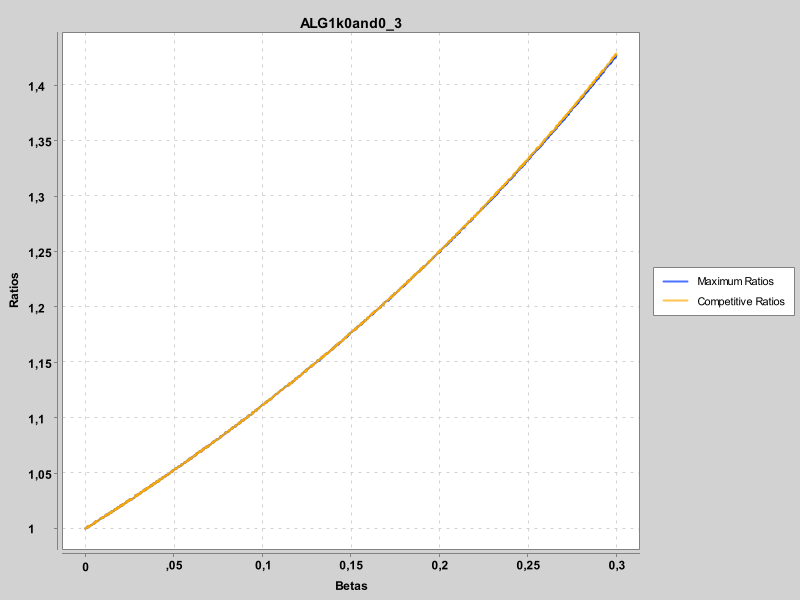
\includegraphics[scale=0.4]{max/ALG1k0and0_3.png}
\end{figure}
\begin{figure}[H]
\caption{Test valore massimo $ALG1_{k}$: $0 \leq \beta < 0.6$}
\centering
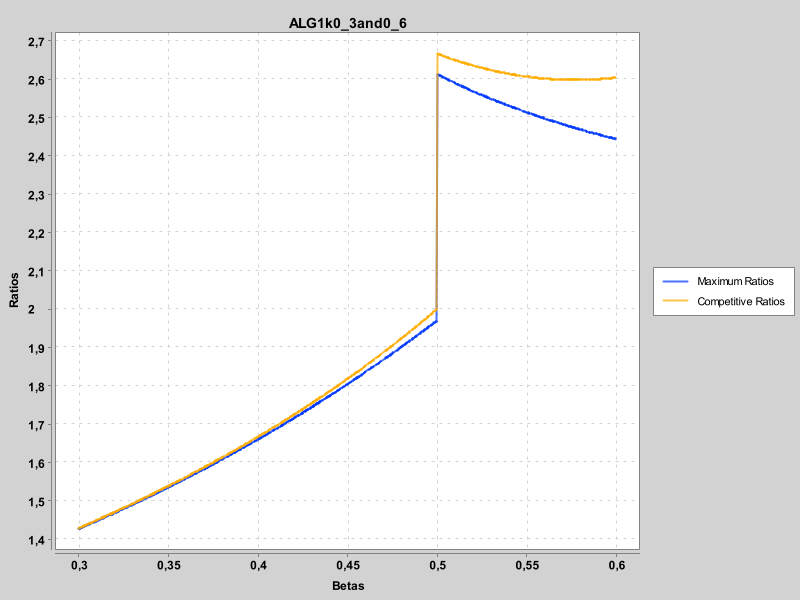
\includegraphics[scale=0.4]{max/ALG1k0_3and0_6.png}
\end{figure}
\begin{figure}[H]
\caption{Test valore massimo $ALG1_{k}$: $0.6 \leq \beta < 0.8$}
\centering
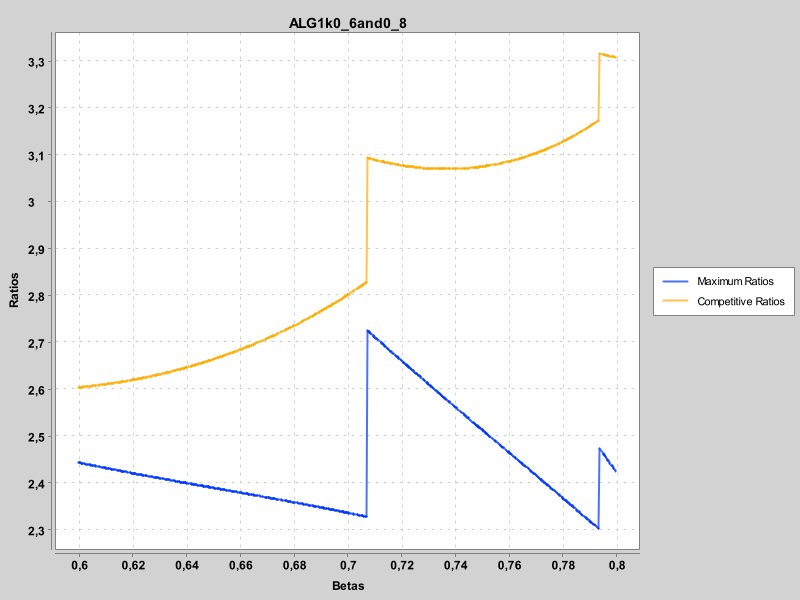
\includegraphics[scale=0.4]{max/ALG1k0_6and0_8.png}
\end{figure}
\begin{figure}[H]
\caption{Test valore massimo $ALG1_{k}$: $0.8 \leq \beta < 1$}
\centering
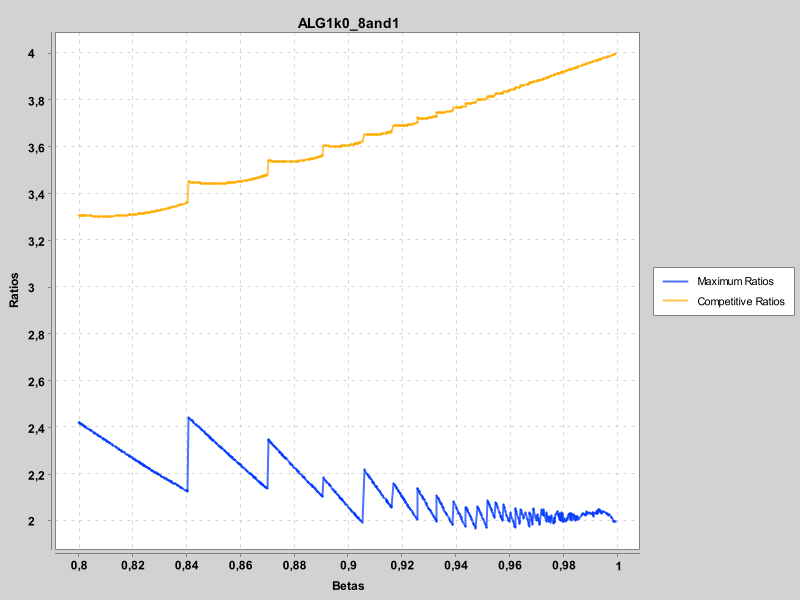
\includegraphics[scale=0.4]{max/ALG1k0_8and1.png}
\end{figure}
\begin{figure}[H]
\caption{Risultati complessivi dei test valore massimo di $ALG1_{K}$}
\centering
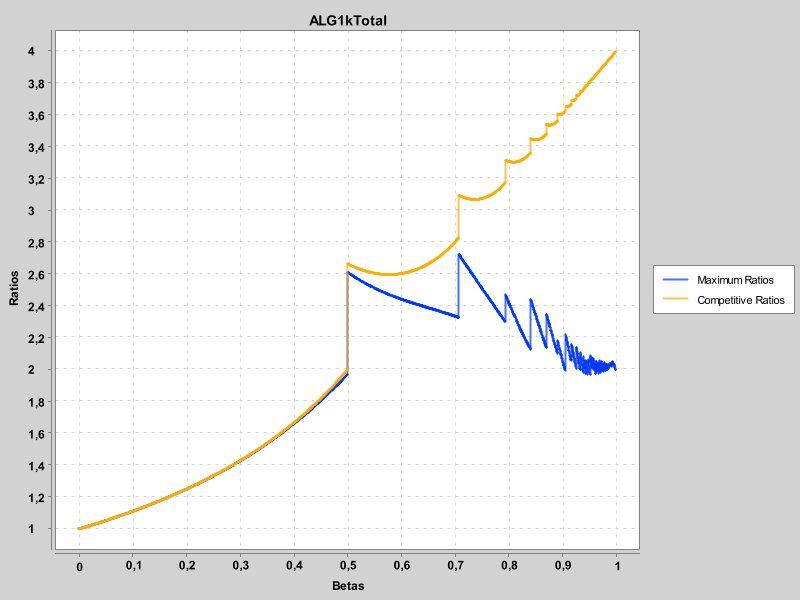
\includegraphics[scale=0.4]{max/ALG1kTotal.png}
\end{figure}
\begin{figure}[H]
\caption{Test caso peggiore $ALG1_{k}$: $0 < \beta < 0.3$}
\centering
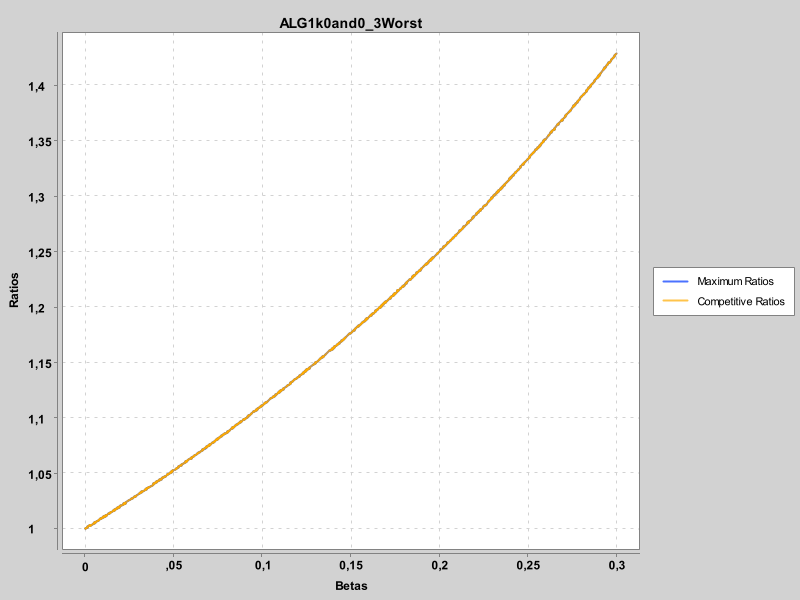
\includegraphics[scale=0.4]{max/ALG1k0and0_3Worst.png}
\end{figure}
\begin{figure}[H]
\caption{Test caso peggiore $ALG1_{k}$: $0 \leq \beta < 0.6$}
\centering
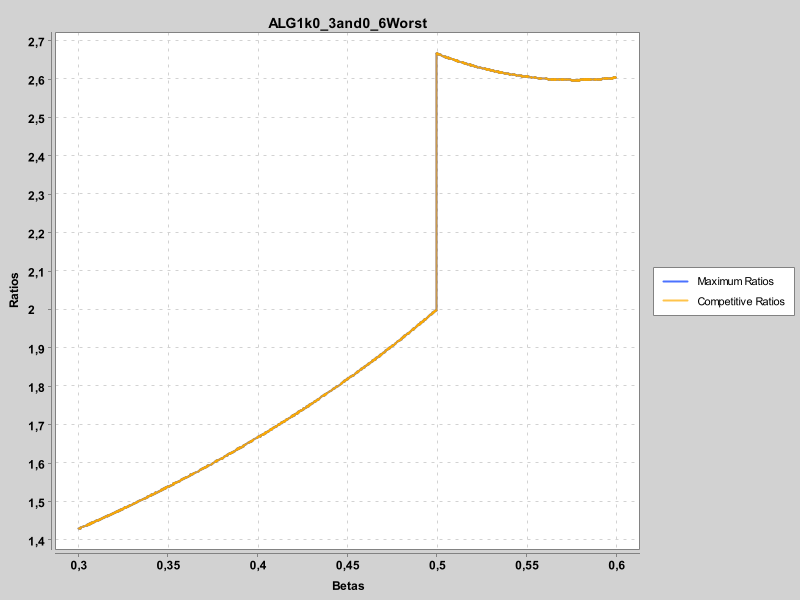
\includegraphics[scale=0.4]{max/ALG1k0_3and0_6Worst.png}
\end{figure}
\begin{figure}[H]
\caption{Test caso peggiore $ALG1_{k}$: $0.6 \leq \beta < 0.8$}
\centering
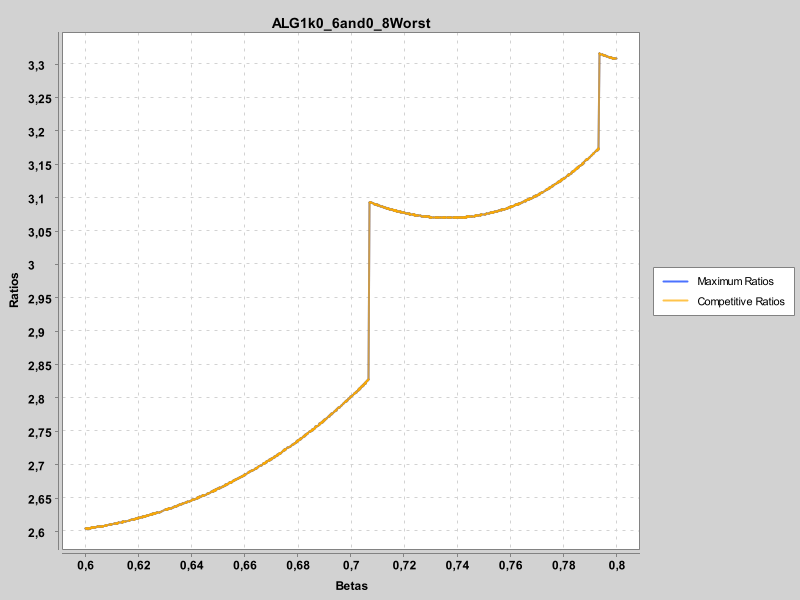
\includegraphics[scale=0.4]{max/ALG1k0_6and0_8Worst.png}
\end{figure}
\begin{figure}[H]
\caption{Test caso peggiore $ALG1_{k}$: $0.8 \leq \beta < 1$}
\centering
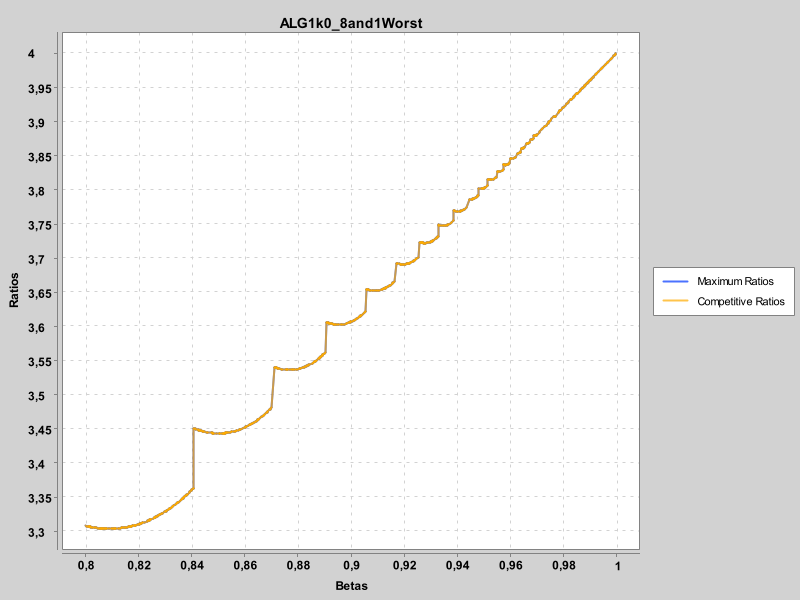
\includegraphics[scale=0.4]{max/ALG1k0_8and1Worst.png}
\end{figure}
\begin{figure}[H]
\caption{Risultati complessivi dei test caso peggiore di $ALG1_{K}$}
\centering
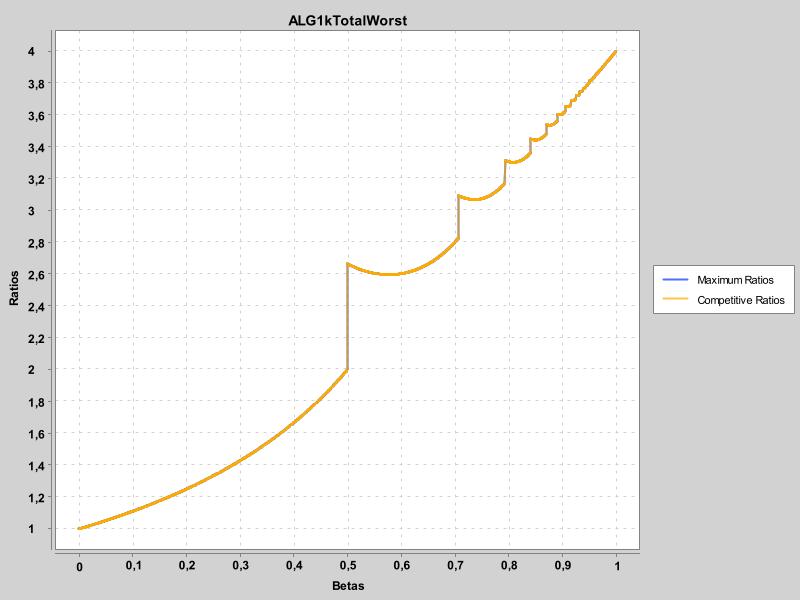
\includegraphics[scale=0.4]{max/ALG1kTotalWorst.png}
\end{figure}

\subsection{$ALG2_{k}$}
\setcounter{figure}{0} 
\renewcommand{\thefigure}{\thesubsection.\arabic{figure}}
\begin{figure}[H]
\caption{Test valore massimo $ALG2_{k}$: $0 < \beta < 0.3$}
\centering
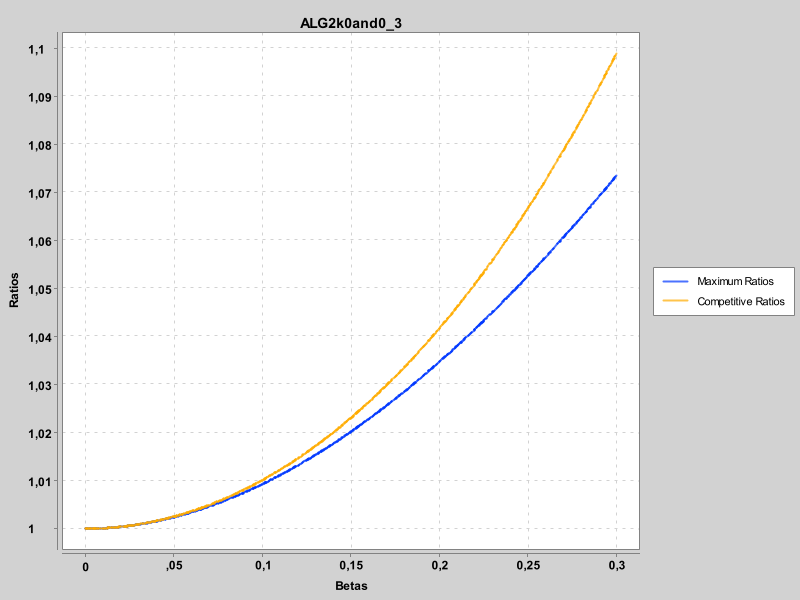
\includegraphics[scale=0.4]{max/ALG2k0and0_3.png}
\end{figure}
\begin{figure}[H]
\caption{Test valore massimo $ALG2_{k}$: $0 \leq \beta < 0.6$}
\centering
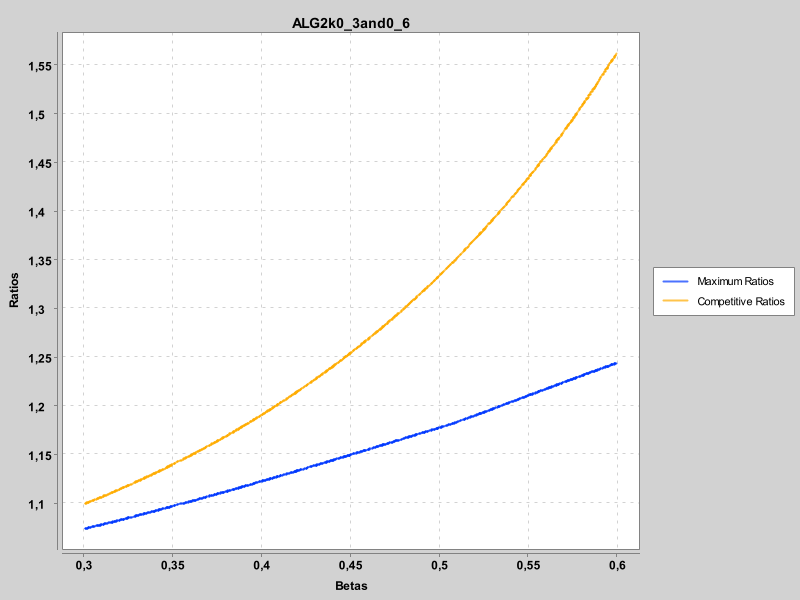
\includegraphics[scale=0.4]{max/ALG2k0_3and0_6.png}
\end{figure}
\begin{figure}[H]
\caption{Test valore massimo $ALG2_{k}$: $0.6 \leq \beta < 0.8$}
\centering
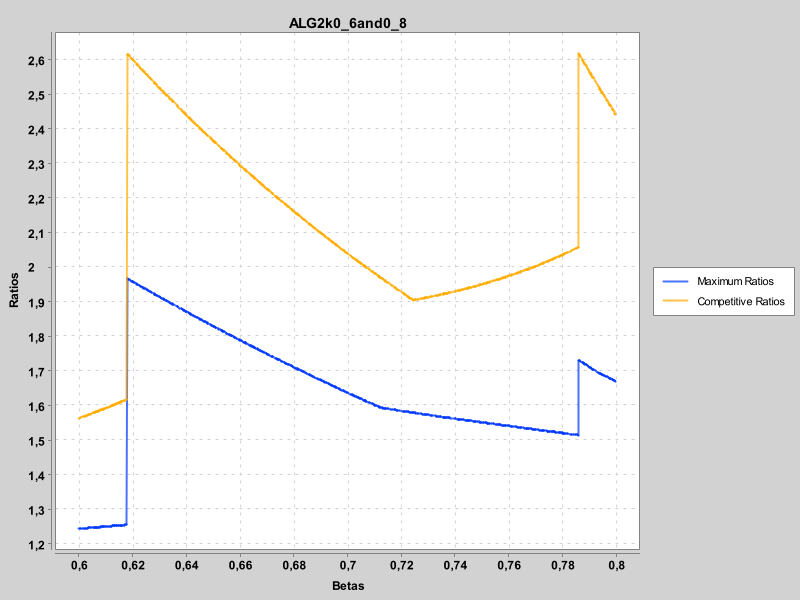
\includegraphics[scale=0.4]{max/ALG2k0_6and0_8.png}
\end{figure}
\begin{figure}[H]
\caption{Test valore massimo $ALG2_{k}$: $0.8 \leq \beta < 1$}
\centering
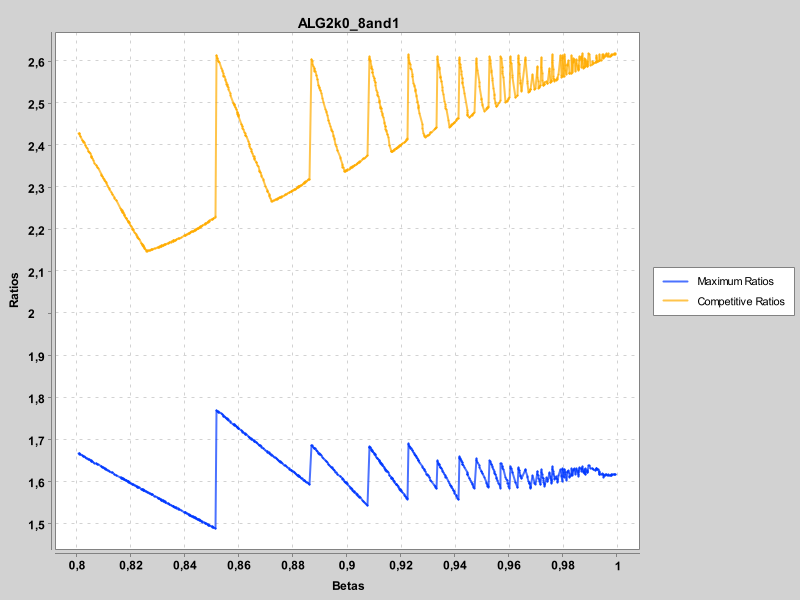
\includegraphics[scale=0.4]{max/ALG2k0_8and1.png}
\end{figure}
\begin{figure}[H]
\caption{Risultati complessivi dei test valore massimo di $ALG2_{k}$}
\centering
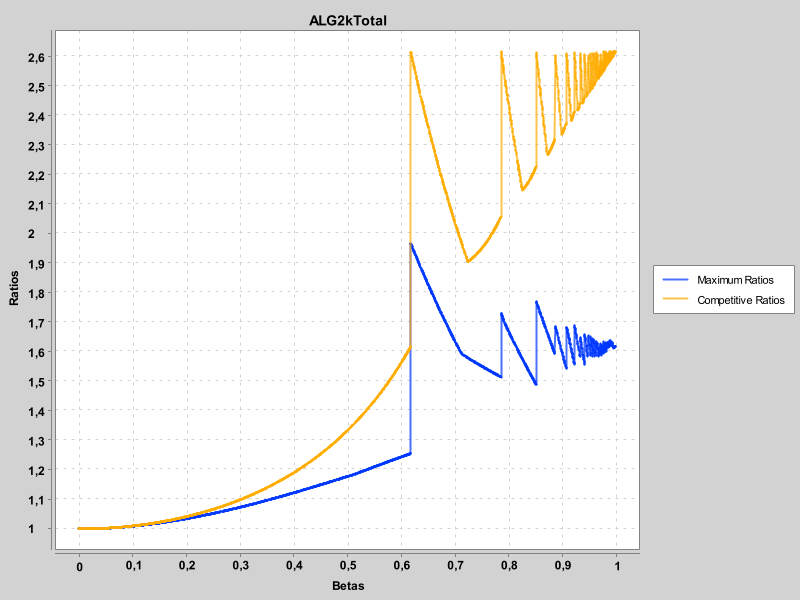
\includegraphics[scale=0.4]{max/ALG2kTotal.png}
\end{figure}
\begin{figure}[H]
\caption{Test caso peggiore $ALG2_{k}$: $0 < \beta < 0.3$}
\centering
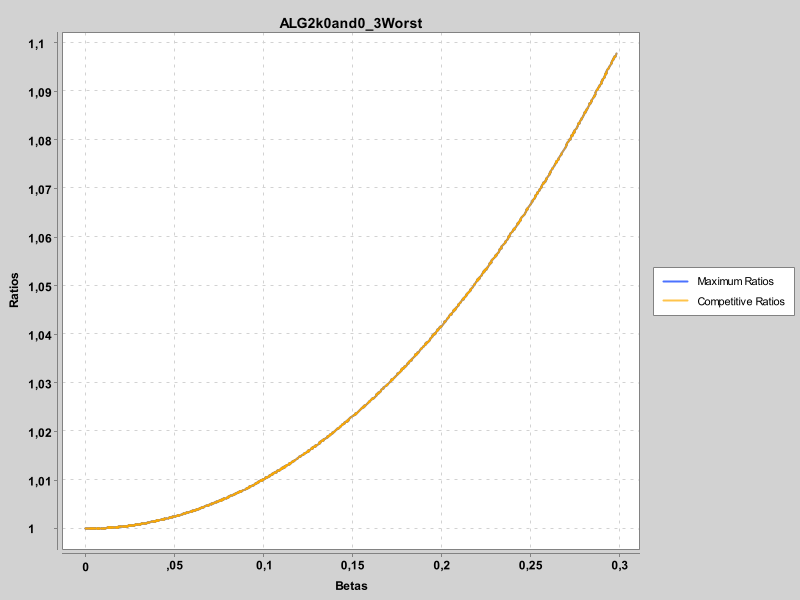
\includegraphics[scale=0.4]{max/ALG2k0and0_3Worst.png}
\end{figure}
\begin{figure}[H]
\caption{Test caso peggiore $ALG2_{k}$: $0 \leq \beta < 0.6$}
\centering
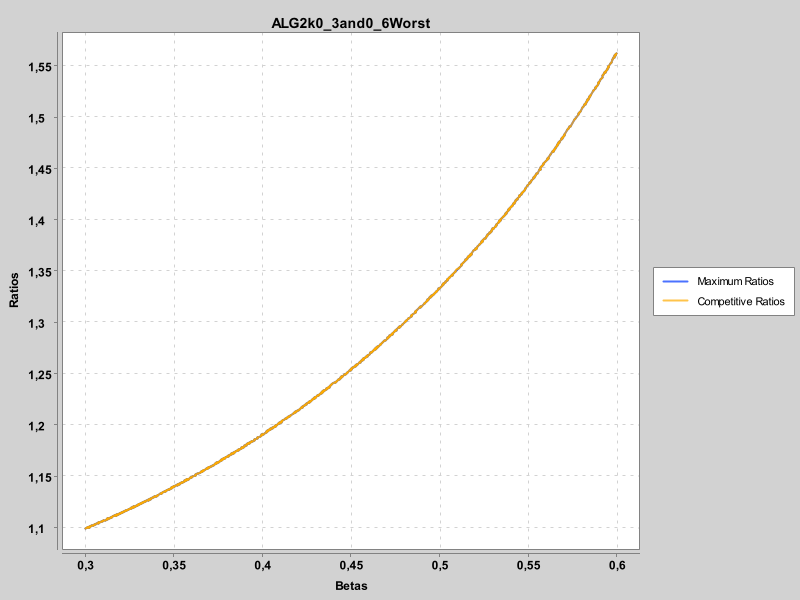
\includegraphics[scale=0.4]{max/ALG2k0_3and0_6Worst.png}
\end{figure}
\begin{figure}[H]
\caption{Test caso peggiore $ALG2_{k}$: $0.6 \leq \beta < 0.8$}
\centering
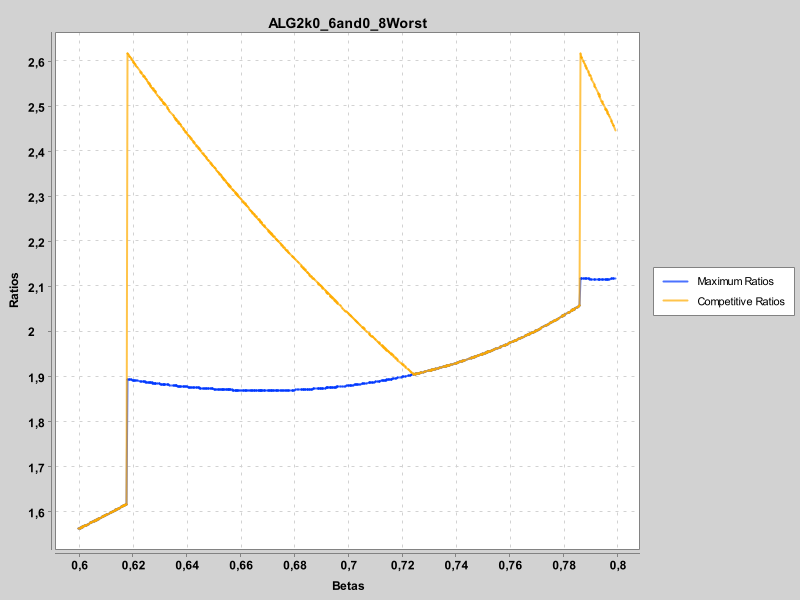
\includegraphics[scale=0.4]{max/ALG2k0_6and0_8Worst.png}
\end{figure}
\begin{figure}[H]
\caption{Test caso peggiore $ALG2_{k}$: $0.8 \leq \beta < 1$}
\centering
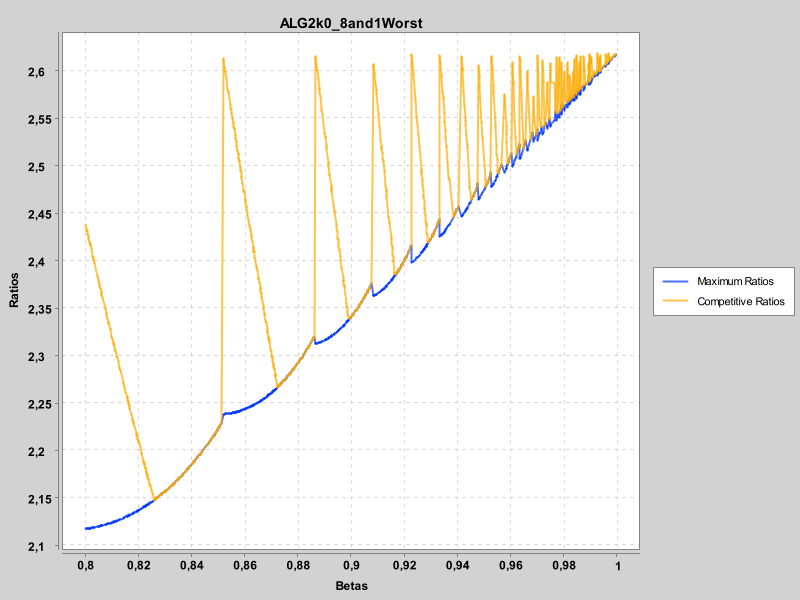
\includegraphics[scale=0.4]{max/ALG2k0_8and1Worst.png}
\end{figure}
\begin{figure}[H]
\caption{Risultati complessivi dei test caso peggiore di $ALG2_{k}$}
\centering
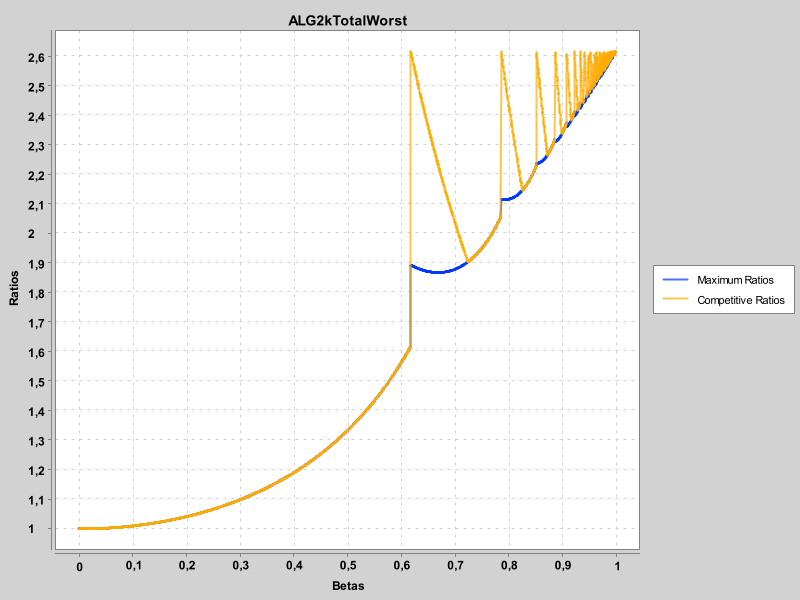
\includegraphics[scale=0.4]{max/ALG2kTotalWorst.png}
\end{figure}

\subsection{$ALG(m)_{k}$}
\setcounter{figure}{0} 
\renewcommand{\thefigure}{\thesubsection.\arabic{figure}}
\begin{figure}[H]
\caption{Test valore massimo $ALG(m)_{k}$: $0 < \beta < 0.3$, $m = 10$}
\centering
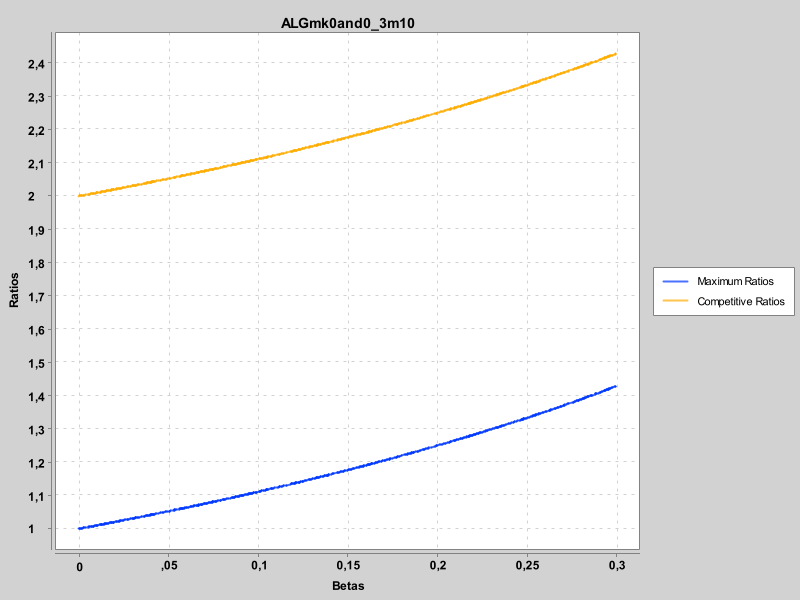
\includegraphics[scale=0.4]{max/ALGmk0and0_3m10.png}
\end{figure}
\begin{figure}[H]
\caption{Test valore massimo $ALG(m)_{k}$: $0 \leq \beta < 0.6$, $m = 10$}
\centering
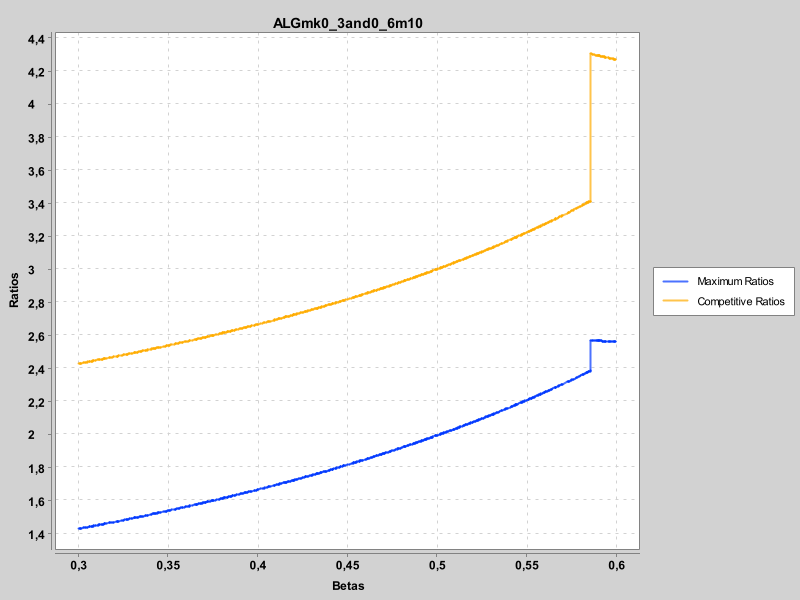
\includegraphics[scale=0.4]{max/ALGmk0_3and0_6m10.png}
\end{figure}
\begin{figure}[H]
\caption{Test valore massimo $ALG(m)_{k}$: $0.6 \leq \beta < 0.8$, $m = 10$}
\centering
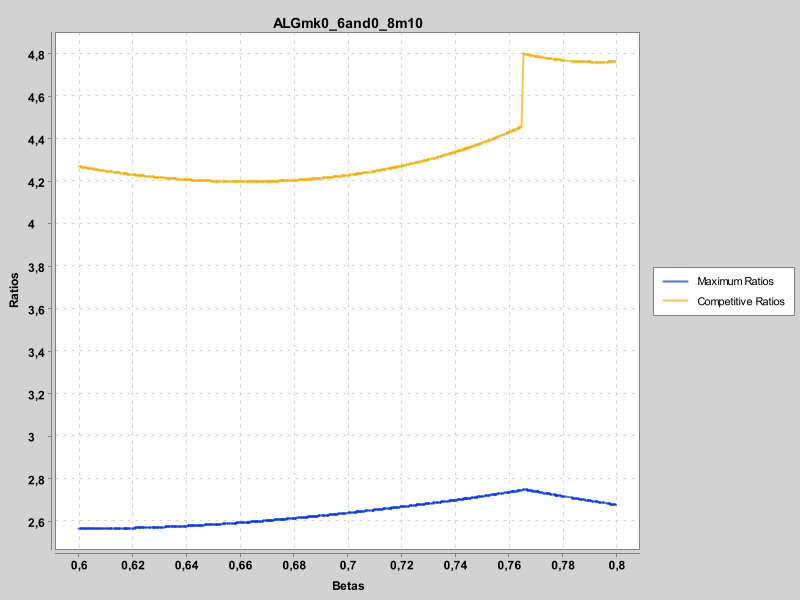
\includegraphics[scale=0.4]{max/ALGmk0_6and0_8m10.png}
\end{figure}
\begin{figure}[H]
\caption{Test valore massimo $ALG(m)_{k}$: $0.8 \leq \beta < 1$, $m = 10$}
\centering
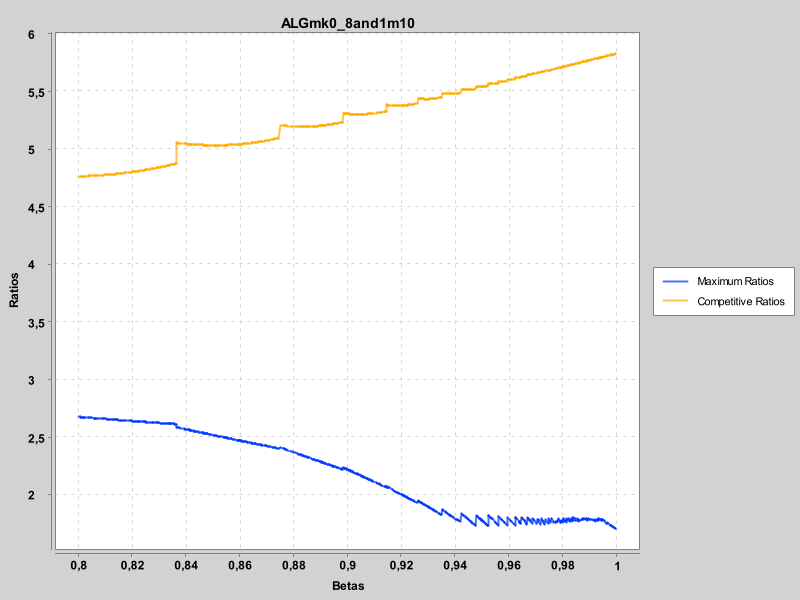
\includegraphics[scale=0.4]{max/ALGmk0_8and1m10.png}
\end{figure}
\begin{figure}[H]
\caption{Risultati complessivi dei test valore massimo di $ALG(m)_{k}$, $m = 10$}
\centering
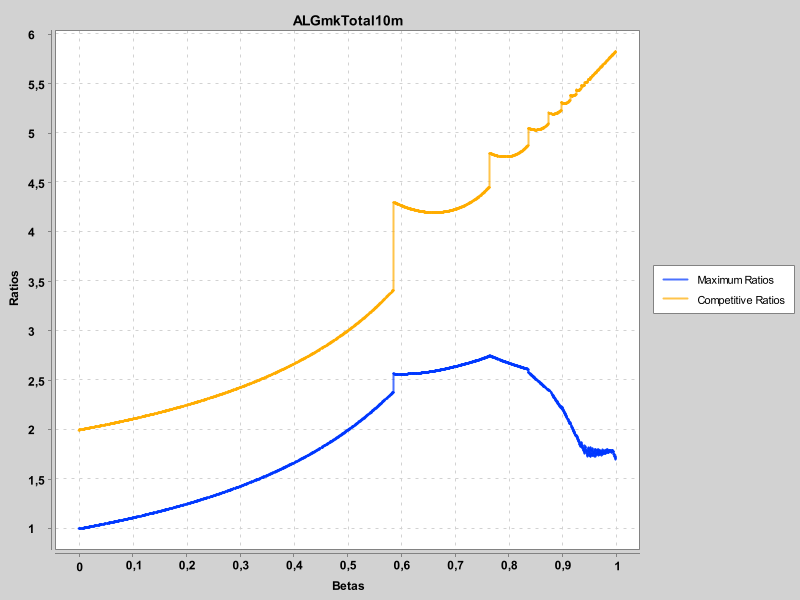
\includegraphics[scale=0.4]{max/ALGmkTotalm10.png}
\end{figure}

\begin{figure}[H]
\caption{Test caso peggiore $ALG(m)_{k}$: $0 < \beta < 0.3$, $m = 10$}
\centering
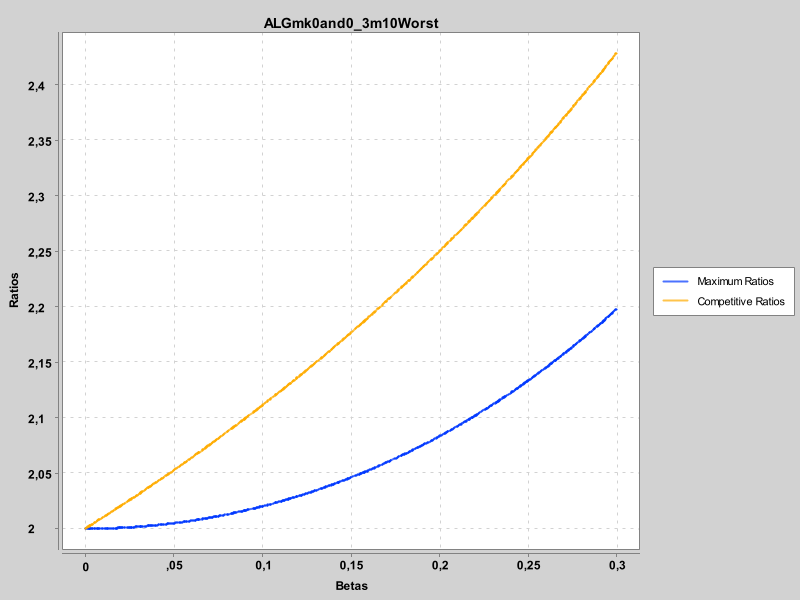
\includegraphics[scale=0.4]{max/ALGmk0and0_3m10Worst.png}
\end{figure}
\begin{figure}[H]
\caption{Test caso peggiore $ALG(m)_{k}$: $0 \leq \beta < 0.6$, $m = 10$}
\centering
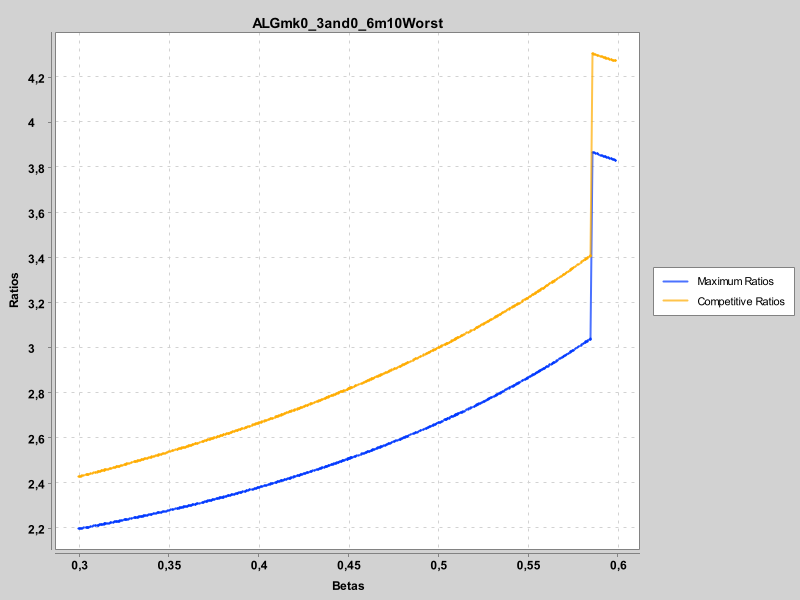
\includegraphics[scale=0.4]{max/ALGmk0_3and0_6m10Worst.png}
\end{figure}
\begin{figure}[H]
\caption{Test caso peggiore $ALG(m)_{k}$: $0.6 \leq \beta < 0.8$, $m = 10$}
\centering
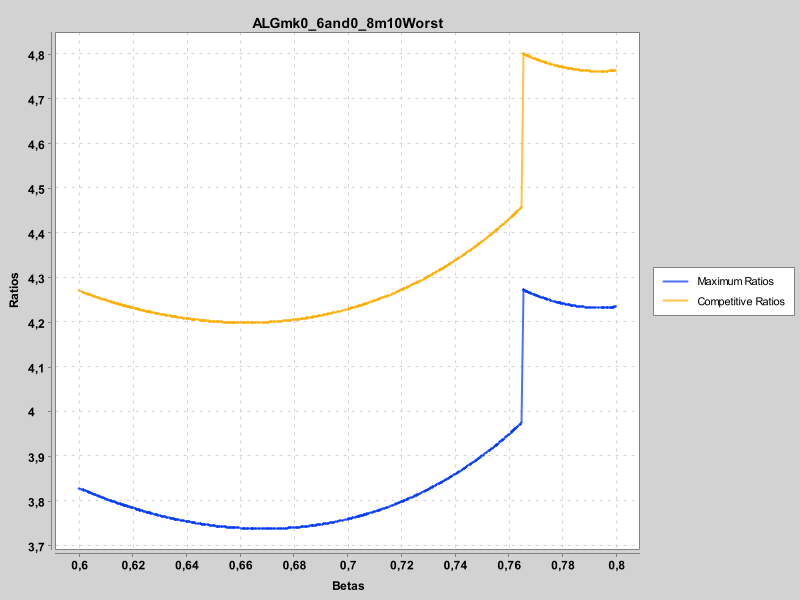
\includegraphics[scale=0.4]{max/ALGmk0_6and0_8m10Worst.png}
\end{figure}
\begin{figure}[H]
\caption{Test caso peggiore $ALG(m)_{k}$: $0.8 \leq \beta < 1$, $m = 10$}
\centering
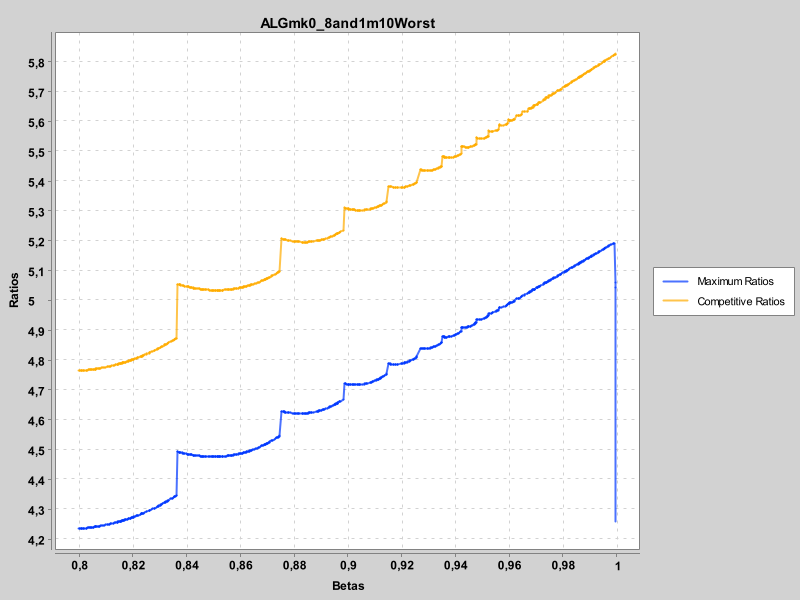
\includegraphics[scale=0.4]{max/ALGmk0_8and1m10Worst.png}
\end{figure}
\begin{figure}[H]
\caption{Risultati complessivi dei test caso peggiore di $ALG(m)_{k}$, $m = 10$}
\centering
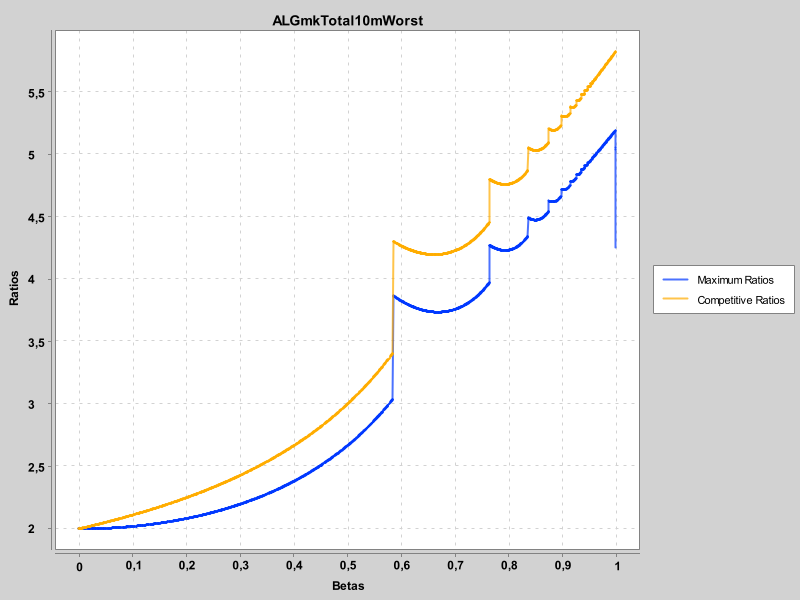
\includegraphics[scale=0.4]{max/ALGmkTotalm10Worst.png}
\end{figure}

\end{document}